%% ****** Start of file apsguide4-2.tex ****** %
%%
%%   This file is part of the APS files in the REVTeX 4.2 distribution.
%%   Version 4.2b of REVTeX, December 2018.
%%
%%   Copyright (c) 2019 The American Physical Society.
%%
%%   See the REVTeX 4.2 README file for restrictions and more information.
%%
\documentclass[twocolumn,secnumarabic,amssymb, nobibnotes, aps, prd]{revtex4-2}
\usepackage{graphicx}
\usepackage{subfigure}
\usepackage{hyperref}
%\usepackage{acrofont}%NOTE: Comment out this line for the release version!
\newcommand{\revtex}{REV\TeX\ }
\newcommand{\classoption}[1]{\texttt{#1}}
\newcommand{\macro}[1]{\texttt{\textbackslash#1}}
\newcommand{\m}[1]{\macro{#1}}
\newcommand{\env}[1]{\texttt{#1}}
\setlength{\textheight}{9.5in}

\begin{document}

\title{Classroom learning dynamics using a cellular automata spatiotemporal model comparing peer instruction and traditional instruction}%

\author{Clarence Ioakim T. Sy}%
\affiliation{National Institute of Physics, University of the Philippines Diliman, Quezon City, Philippines}%

\author{Ranzivelle Marianne L. Roxas-Villanueva}%
\affiliation{Institute of Physics, University of the Philippines Los Ba\~{n}os, Laguna, Philippines}%

\author{Johnrob Y. Bantang}%
\email[Corresponding author: ]{jybantang@up.edu.ph}
\affiliation{National Institute of Physics, University of the Philippines Diliman, Quezon City, Philippines}%

\date{June 2025}%

\begin{abstract}
    Peer instruction (PI) has recently become one of the popular means of classroom instruction in Physics Education.
    Such instruction method is vastly different from how classes are traditionally handled where the instructor conducts a lecture for the entire duration of the class.
    In this study, we model the transfer of knowledge within the class as a probabilistic cellular automata model and investigate the effects of different factors such as seating arrangements, size, learning rate, and heterogeneity on the classes' overall learning efficiency in peer instruction.
    We compared the learning efficiency between traditional instruction (TI) and peer instruction (PI). 
    We found that larger class sizes sway the advantage towards traditional instruction, while increased learning rate heterogeneity favors PI.
    Additionally, an increase in the students' effective learning rate benefits both TI and PI but in different ways.
    Classes under traditional instruction were found to have two stages of learning when heterogeneity was introduced: a fast initial stage and a slow final stage.
    On the other hand, learning trends in PI were generally unaffected by heterogeneity, having similar effects with the other factors we considered.
    Among the seating arrangements (SAs) we considered for PI, the inner corner SA performed the best.
    This result differs from previous studies where they found that the outer corner SA performed the best.
    The difference stems from the simplifications made in this model.
    We did not consider the orientation factor of each student, resulting in an isotropic system.
    Our model also uses binary values and does not consider the effect of aptitude similarity that have been described in previous studies. 
    Despite these simplifications, our findings generally agree with previous studies and existing practices that PI performs similarly or better than traditional instruction and that a mix of traditional instruction and PI would be the optimal method of instruction.
    We offer insights based on the qualitative results of the model.
\end{abstract}

\maketitle
\tableofcontents

\section{Introduction}

%    Literature discussing peer instruction, especially for physics often cites Mazur's work \textit{Peer Instruction: A User's Manual} .
%    In this book, Mazur recounts how he observed a disconnect between students' ability to answer quantitative and conceptual questions in physics.
    Peer instruction (PI)--an increasingly popular method of instruction--attempts to solve a disconnect between students' ability to answer quantitative and conceptual questions, particularly in physics subject matters~\cite{mazur1997peer,mazur1999}.
%    He concluded that this resulted from the students' approach of memorizing problem solving algorithms, even if they might not always apply to a given problem.
	Such disconnect is said to be attributed to the typical approach of memorizing physics problem patterns and applying the same solution patterns regardless of their potential non-applicability.
%    Peer Instruction (PI) as a method of instruction aims to address this issue.
    The PI method forces students to think critically and to engage with peers guided by the learning material as opposed to simply absorbing the information from lectures given by the instructor as in the traditional mode of instruction (TI).
    The method's effectivity has been shown not only in high school physics settings, but also in other disciplines and higher education settings~\cite{johnson2008active,fagen2000factors,fagen2002peer}.

%%%%%%%%%%%%%%%
%%    \subsection{Difference of Peer Instruction from Traditional Instruction}

%    There are many ways to implement PI in the classroom.
%    The method outlined by Mazur~\cite{mazur1997peer} involves the instructor giving a short lecture on a topic, followed by a multiple choice question (MCQ) that the students answer individually.
%    The students then discuss their answers with their peers before answering an MCQ again.
%    Variations can be made depending on the class set up and the instructor.
    
    The PI method as outlined by Mazur and Somers~\cite{mazur1997peer} typically involves an instructor giving a short lecture on the topic, followed by a multiple-choice question (MCQ) that the student answer individually.
    PI emphasizes on the next phases of instruction which involve repeated cycle of students sharing their answers to the MCQ and discussing them with peers, usually until they get the concepts right.
    This part makes PI method student centric requiring the instructor to intervene with slightly modified steps to adjust to the needs of the class.
    As long as the same learning objectives are tackled, the instructor can choose variations in the method~\cite{smith2009peer} such as the multiplicity of the peer sharing and discussion phase, decide levels of requirements and/or evaluation~\cite{crouch2001peer}, provide different MCQ sets, or even give a short lecture to ensure clarity of concepts~\cite{lasry2008peer}.
    The PI thus contrasts highly against the traditional method (TI) with which the instructor giving a lecture for the entire duration of the class with minimal opportunity of in-class peer interactions among the students.
    
%    This is in stark contrast with how traditional instruction (TI) is conducted where the instructor often just gives a lecture for the entire duration of the class.
%    PI is meant to be student centric, meaning that the instructor is expected to make differences to the steps outlined above to adjust to the class's needs.
%    The MCQs can be graded or ungraded \cite{crouch2001peer}, the instructor can choose to give multiple MCQs and peer discussion opportunities during one class, or the instructor can choose to give a different MCQ after the discussion as long as it still tackles the same learning objective \cite{smith2009peer}.
%    If only a few students answer the MCQ correctly, the instructor can even give a short lecture to clarify the concept \cite{lasry2008peer}.

%%%%%%%%%%%%%%%
%%    \subsection{Benefits of PI}

    Despite the de-emphasis on problem-solving in PI lectures, students' quantitative problem-solving skills were not compromised and was even improved compared to traditional instruction in some cases.
    PI was also shown to significantly decrease the number of of students with extremely low scores \cite{crouch2001peer}.
    This is consistent with findings of other studies \cite{lasry2008peer,thacker1994comparing}.
    Similarly, students' conceptual understanding of the lessons also improved.
    This holds true for both in-class concept tests and end-of-semester exams \cite{crouch2001peer}.

    Smith, et. al \cite{smith2009peer} modified the PI method to make sure that students were not copying off of each other. After the first MCQ, he did not show the class's answer statistics and used a pair of isomorphic questions for the MCQs before and after the peer discussion section. Isomorphic questions are questions that tackle the same learning objectives but have different "cover stories".
    They also found that even in groups whose members were not able to answer the first MCQ, students were able to get the correct answer for the second MCQ.
    This contradicts the transmissionist view of PI where students only learn from other students who already know the lesson.
    The study provides evidence that PI can be viewed as constructivist where students learn on their own through discussion and not simply from hearing the correct answer.

    In addition to those mentioned above Lasry, et. al. \cite{lasry2008peer} showed that PI is not necessarily dependent on background knowledge. They found that students in under PI performed as well as or better than those under TI despite the former having less background knowledge.
    They also found the PI greatly reduced the number of students who dropped the course.
    An older paper by Tobias \cite{tobias1990they} suggests that this could be because of the shift of focus of PI from competition and skill performance to cooperative learning and conceptual understanding.


\section{Existing Mathematical Models of PI}

    Although there are some mathematical models for learning, the ones that describe learning in the classroom are few and far in between - even more so for those that model PI.

    Roxas et al. \cite{roxas2010seating} used actual assessment results to train a neural network to map student interactions in PI classrooms. 
    Using this neural network, they were able to characterize information transfer and investigate the effects of group homogeneity. 
    Their study also investigated the optimal seating arrangement for students under PI methods based on their aptitude.
    In their paper, the measure of students' improvement was calculated via the Hake gain as shown in Equation~\ref{eq: hake gain} \cite{hake1998}.
    They also used the output/input ratio (O/I), which was the ratio of second assessment scores vs first assessment scores, to gauge student improvement.
    However, it should be noted that O/I values tend to be biased towards low-scoring students.
    \begin{equation}
        \label{eq: hake gain}
        \langle g \rangle = \frac{\langle 2^{\text{nd}}\text{ assessment} - 1^{\text{st}}\text{ assessment} \rangle}{\langle 1 - 1^{\text{st}}\text{ assessment} \rangle}
    \end{equation}

    The results of their study show that the outer corner seating arrangement (SA) performed the best, followed by inner corner, then random, then center (see Figure~\ref{fig:PI SAs} for SA visualizations).
    In simulated classrooms, each with 64 students and 10 classrooms in total, they found that homogenous classrooms with low aptitudes have significantly higher O/I values.
    This means that low aptitude students benefit the most from being grouped together.

    \begin{figure}[htbp!]
        \centering
        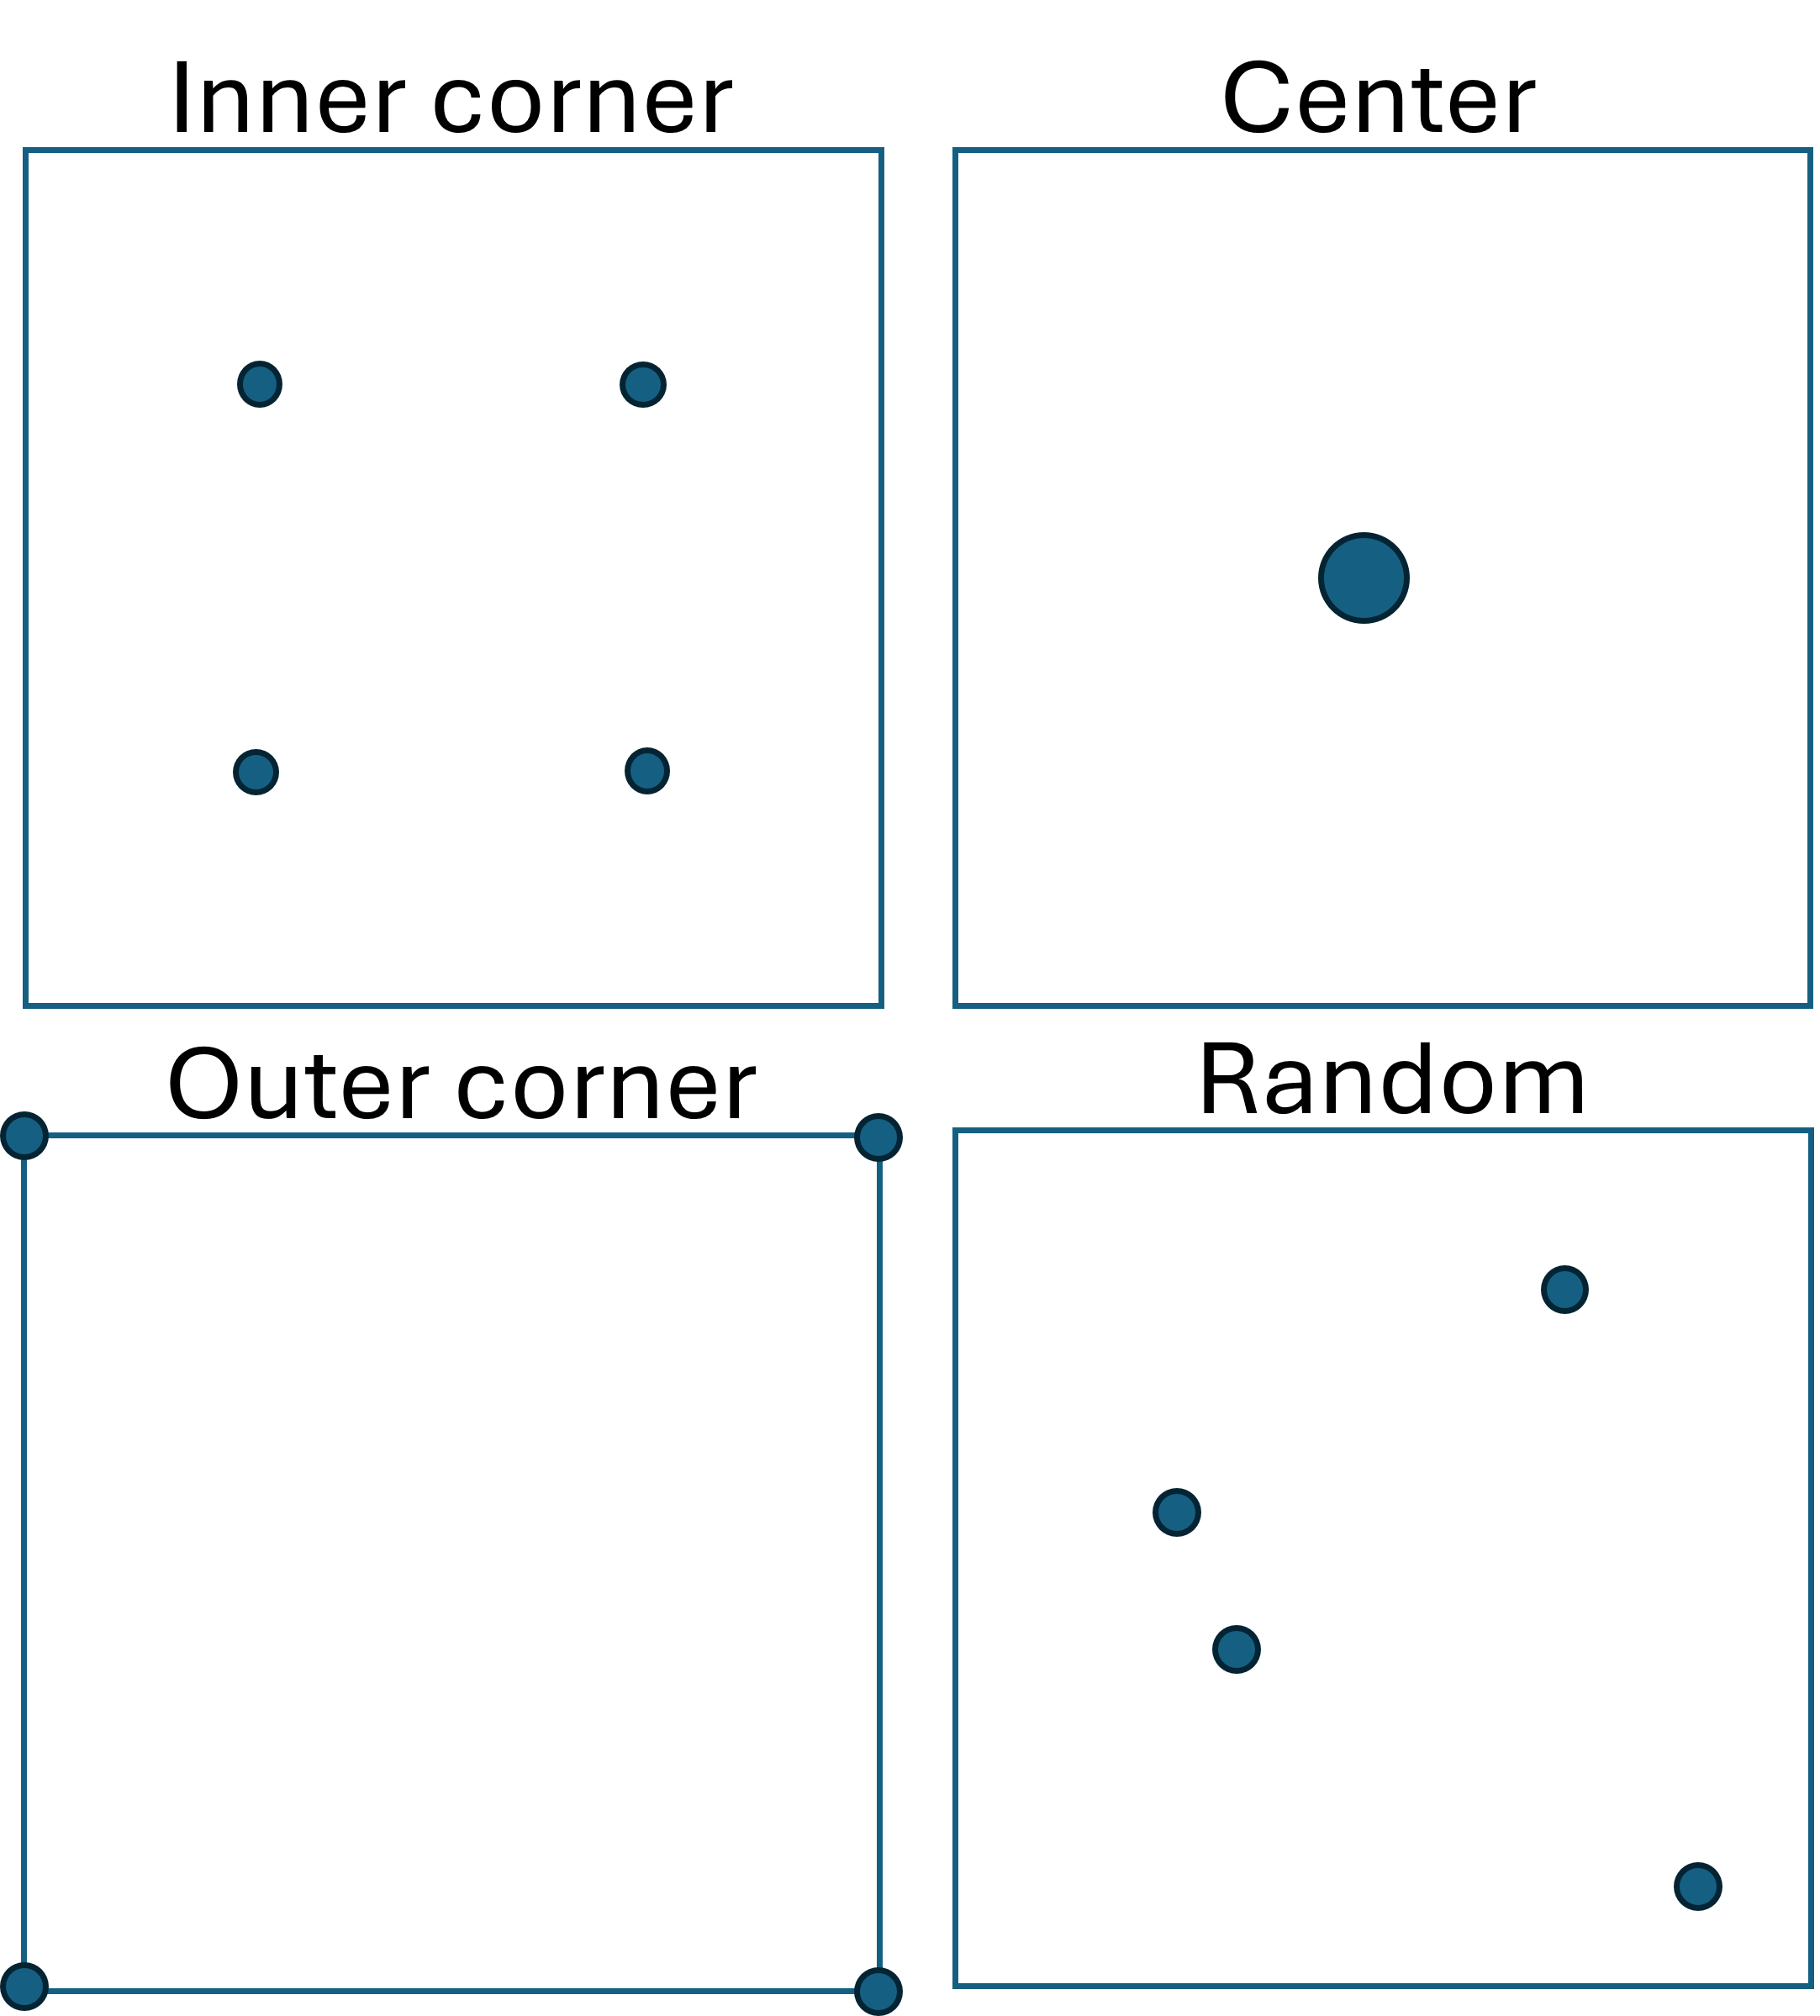
\includegraphics[width=0.40\textwidth]{figures/PI SAs.png}
        \caption{Seating arrangements considered for PI. Dots represent position of high aptitude students.}
        \label{fig:PI SAs}
    \end{figure}

    Nitta \cite{nitta2019mathematical} gives us a few existing models that model PI. 
    One of the models that was presented is a generalized Ising Model by Bordogna and Albano \cite{bordogna2001theoretical,bordogna2003simulation} where they consider three sources of information for the student to learn from: teacher instruction, peer interaction, and bibliographic materials (books, lecture notes, etc.)
    Their model shows that students learn more when they engage discussions with their peers than those who only listen to lectures.
    They also show that group structure affects student learning, and that low aptitude students may learn at the expense of high aptitude peers - a transmissionist view of PI.

    Nitta also presents a model by Pritchard et al \cite{pritchard2008mathematical} where PI is modeled as a set differential equations that is dependent on the probability of students learning to stick (memory model, Equation~\ref{eq:memory model}) and the ability for students to associate new learnings from old knowledge via logistic differential equation (connectedness model, Equation~\ref{eq:connectedness model}.)
%%
    The Memory model requires
    \begin{equation}
        \label{eq:memory model}
        \frac{dU_T(t)}{dt} = -\alpha_m U_T(t)
    \end{equation}
%%
    while the Connectedness model requires
    \begin{equation}
        \label{eq:connectedness model}
        \frac{dU_T(t)}{dt} = -\alpha_c U_T(t)K_T(t),
    \end{equation}
%%
    where knowledge is taken to grow at a uniform rate, as in the Tutoring model:
    \begin{eqnarray}
        K_T(t) &=& \alpha_{tu}t + K_T(0) \label{eq:tutoring model} \\
        U(t) + K(T) &=& 1
    \end{eqnarray}
%%
    In these equations $U(T)$ and $K(T)$ are the unknown and known knowledge domains respectively.
    The parameters $\alpha_m$, $\alpha_c$, and $\alpha_{tu}$ are the corresponding rates for the memory model, connectedness model, and tutoring model 

    In deriving their own model of PI, Nitta arrived at analytic equations similar to the Hake gain (Equation~\ref{eq: hake gain}) to evaluate the effectiveness of PI for a concept test question (Equation~\ref{eq: PIE}) and Pritchard's connectedness model (Equation~\ref{eq:connectedness model}) to model students' learning after each MCQ (Equation~\ref{eq: nitta model}).

    \begin{equation}
        \label{eq: PIE}
        \eta(q) \equiv \frac{\rho_2(q;c)-\rho_1(q;c)}{1-\rho_1(q;c)}
    \end{equation}

    \begin{equation}
        \label{eq: nitta model}
        \rho_2 = \rho_1 +\rho_1(1-\rho_1)
    \end{equation}

    Comparing their equations to data, they concluded that these metrics and equations roughly agree with the data and could give us insights on the learning dynamics of the classroom.

    The process of PI is complex, with many interacting components.
    Existing models are either predictive, as in the case of the neural network modeling of Roxas et al. \cite{roxas2010seating} or lack the spatial aspect of the process as with the differential equations of Pritchard \cite{pritchard2008mathematical} and Nitta \cite{nitta2019mathematical}.
    While Bordogna et al. \cite{bordogna2001theoretical,bordogna2003simulation} present to us a dynamical model in their generalized Ising model, it lacks some of the aspects of PI we'd like to consider like seating arrangements, students' learning rate, and heterogeneity.

    We propose that a probabilistic cellular automata model can be used to study the spatiotemporal dynamics of both PI and traditional instruction when incorporating these different aspects into the model.
    We previously used a probabilistic cellular automata to model the classroom \cite{SelfSPP}, the results of which were presented in the 42$^{\text{nd}}$ Samahang Pisika ng Pilipinas Conference in July 2024.
    The findings presented in the paper are also presented in this study as part of the results.

\section{Modelling The Classroom As A Probabilistic Cellular Automaton}

    We use a probabilistic cellular automata (PCA) model to simulate the learning process in the classroom.
    In this PCA model, each cell in the automaton represents a student where each student is assigned a learning rate $\lambda_{i,j}$ to describe how fast they learn as an individual.
    The state of each cell represents their aptitude $s_{i,j}=\lbrace\text{unlearned},\text{learned}\rbrace=\lbrace0,1\rbrace$.
    We assign the neighborhood to be an outer totalistic Moore neighborhood of radius $r=1$ and define the boundary conditions to be fixed wherein the grid does not wrap around itself and $s_{i,j}=0 \text{ for }i,j\notin[1,L]$.
    For each time step, we find the probability of a student to learn and update the state of the student based on this probability.
    The probability of a student to learn is calculated differently for traditional instruction and peer instruction.

    \subsection{Update Rules for Traditional Instruction (TI)}

        For traditional instruction, the probability of a student to learn in each time step ($P_{i,j}$) is given by:

        \begin{equation}
            P_{i,j} = \lambda_{i,j}\rho_0
        \end{equation}

        where

        $P_{i,j} \in [0,1]$ is the probability of student $c_{i,j}$ to learn in each time step, 

        $\lambda_{i,j} \in [0,1]$ is the learning rate of student $c_{i,j}$

        $\rho_{0} \in [0,1]$ is the probability of $c_{i,j}$ to learn from the teacher based on their relative position from the teacher.

        We consider the case that students have heterogeneous learning rates $\lambda_{i,j}=\lambda_0 \pm \delta\lambda$ where $\lambda_0=0.5$.
        This allows us to investigate the effects of student heterogeneity on the classroom's learning dynamics.

        Having a positional learning coefficient $\rho_{i,j}$ allows us to model a classroom where students closer to the teacher in front learn faster than those farther away or vice versa.
        However, for this research, we only consider the case such that $\rho_{i,j} = \rho_0 \forall i,j$.

        The numerical procedure is outlined in Figure~\ref{fig:TI flowchart}.
        Each simulation for the TI model starts with all students unlearned.

        \begin{figure}[htbp!]
            \centering
            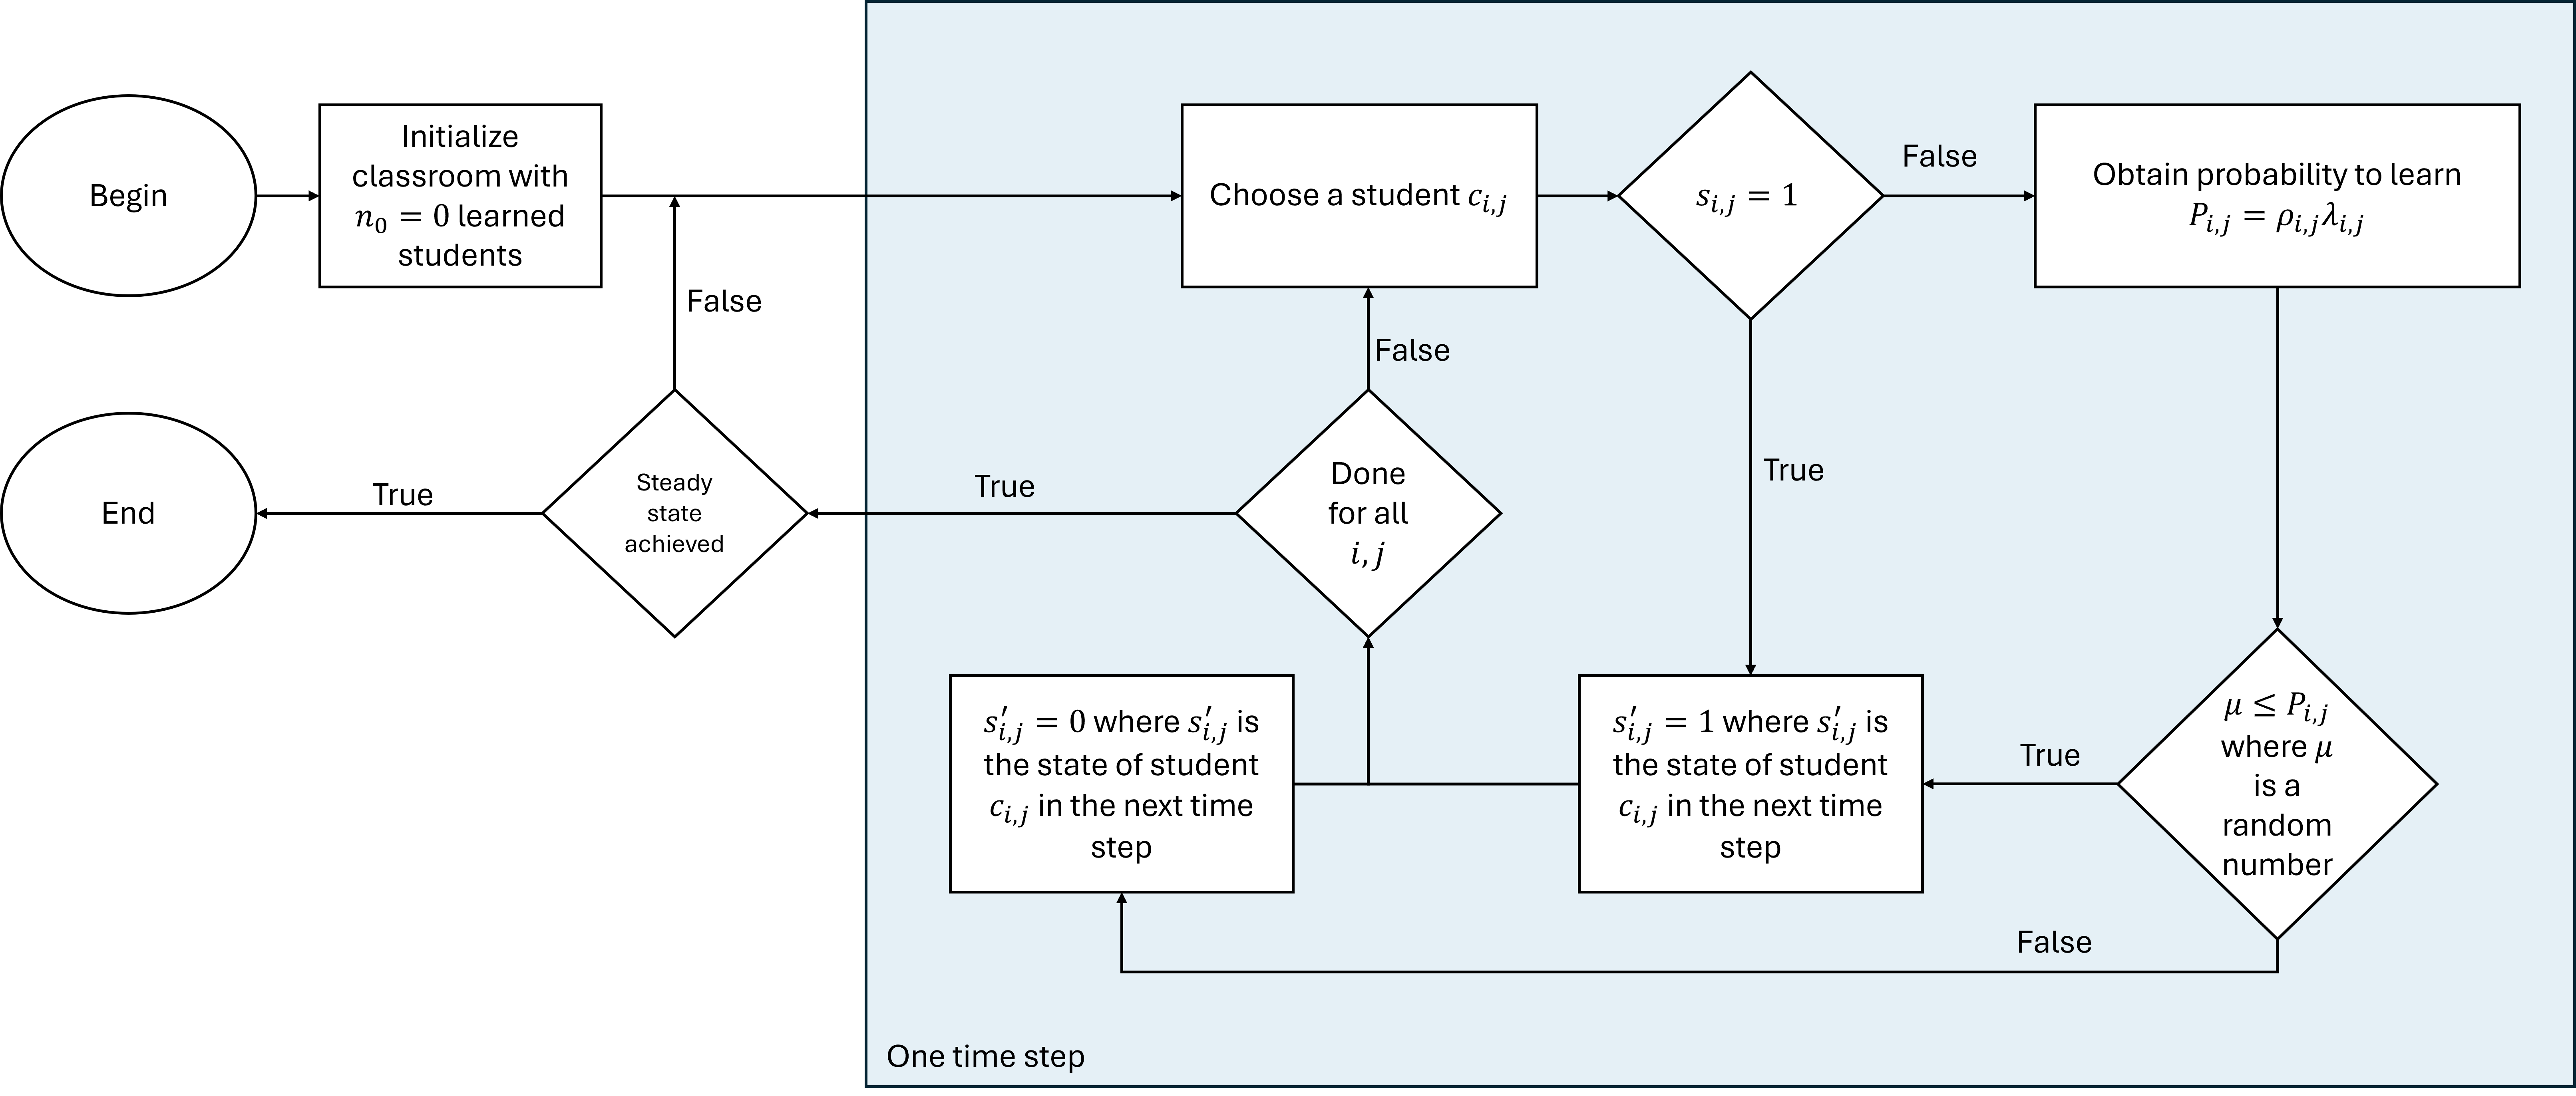
\includegraphics[width=0.45\textwidth]{figures/2DBPCA TI Flowchart.png}
            \caption[Traditional instruction simulation flowchart]{Numerical process for simulation of 2D BPCA for traditional instruction.}
            \label{fig:TI flowchart}
        \end{figure}

    \subsection{Update Rules for Peer Instruction (PI)}

        In contrast to TI, the probability of a student to learn in each time step for PI is additionally dependent on the student's neighbors and their states. The probability of a student to learn in each time step ($P_{i,j}$) is given by:

        \begin{equation}
            \label{eq:BPCA PI learning probability}
                P_{i,j} = 1 - \prod_{\forall \delta i, \delta j}{\lbrack1-(\lambda_{i,j})(\rho_{\delta i, \delta j})(s_{i+\delta i, j+\delta j})}\rbrack
        \end{equation}
        
        where
        
        $P_{i,j} \in [0,1]$ is the probability of student $c_{i,j}$ to learn in each time step, 
        
        $\lambda_{i,j} \in  [0,1]$ is the learning rate of student $c_{i,j}$. We consider the case that students have heterogeneous learning rates $\lambda_{i,j}=\lambda_0 \pm \delta\lambda$ where $\lambda_0=0.5$.
        
        $\rho_{\delta i, \delta j} \in [0,1]$ is the probability of $c_{i,j}$ to learn from their neighbors in seats $\lbrace c_{i+\delta i, j+\delta j} \forall \delta i, \delta j \in \lbrace -1,0,1 \rbrace \rbrace$ solely based from their relative positions with each other, and
        
        $s_{i+\delta i, j+\delta j} = \lbrace\text{unlearned, learned}\rbrace=\lbrace 0,1 \rbrace$ are the neighbors' aptitude level.

        The numerical procedure is outlined in Figure~\ref{fig:PI flowchart}.
        Each simulation for the PI model starts with only four learned students $n_0 = 4$.

        \begin{figure}[htbp!]
            \centering
            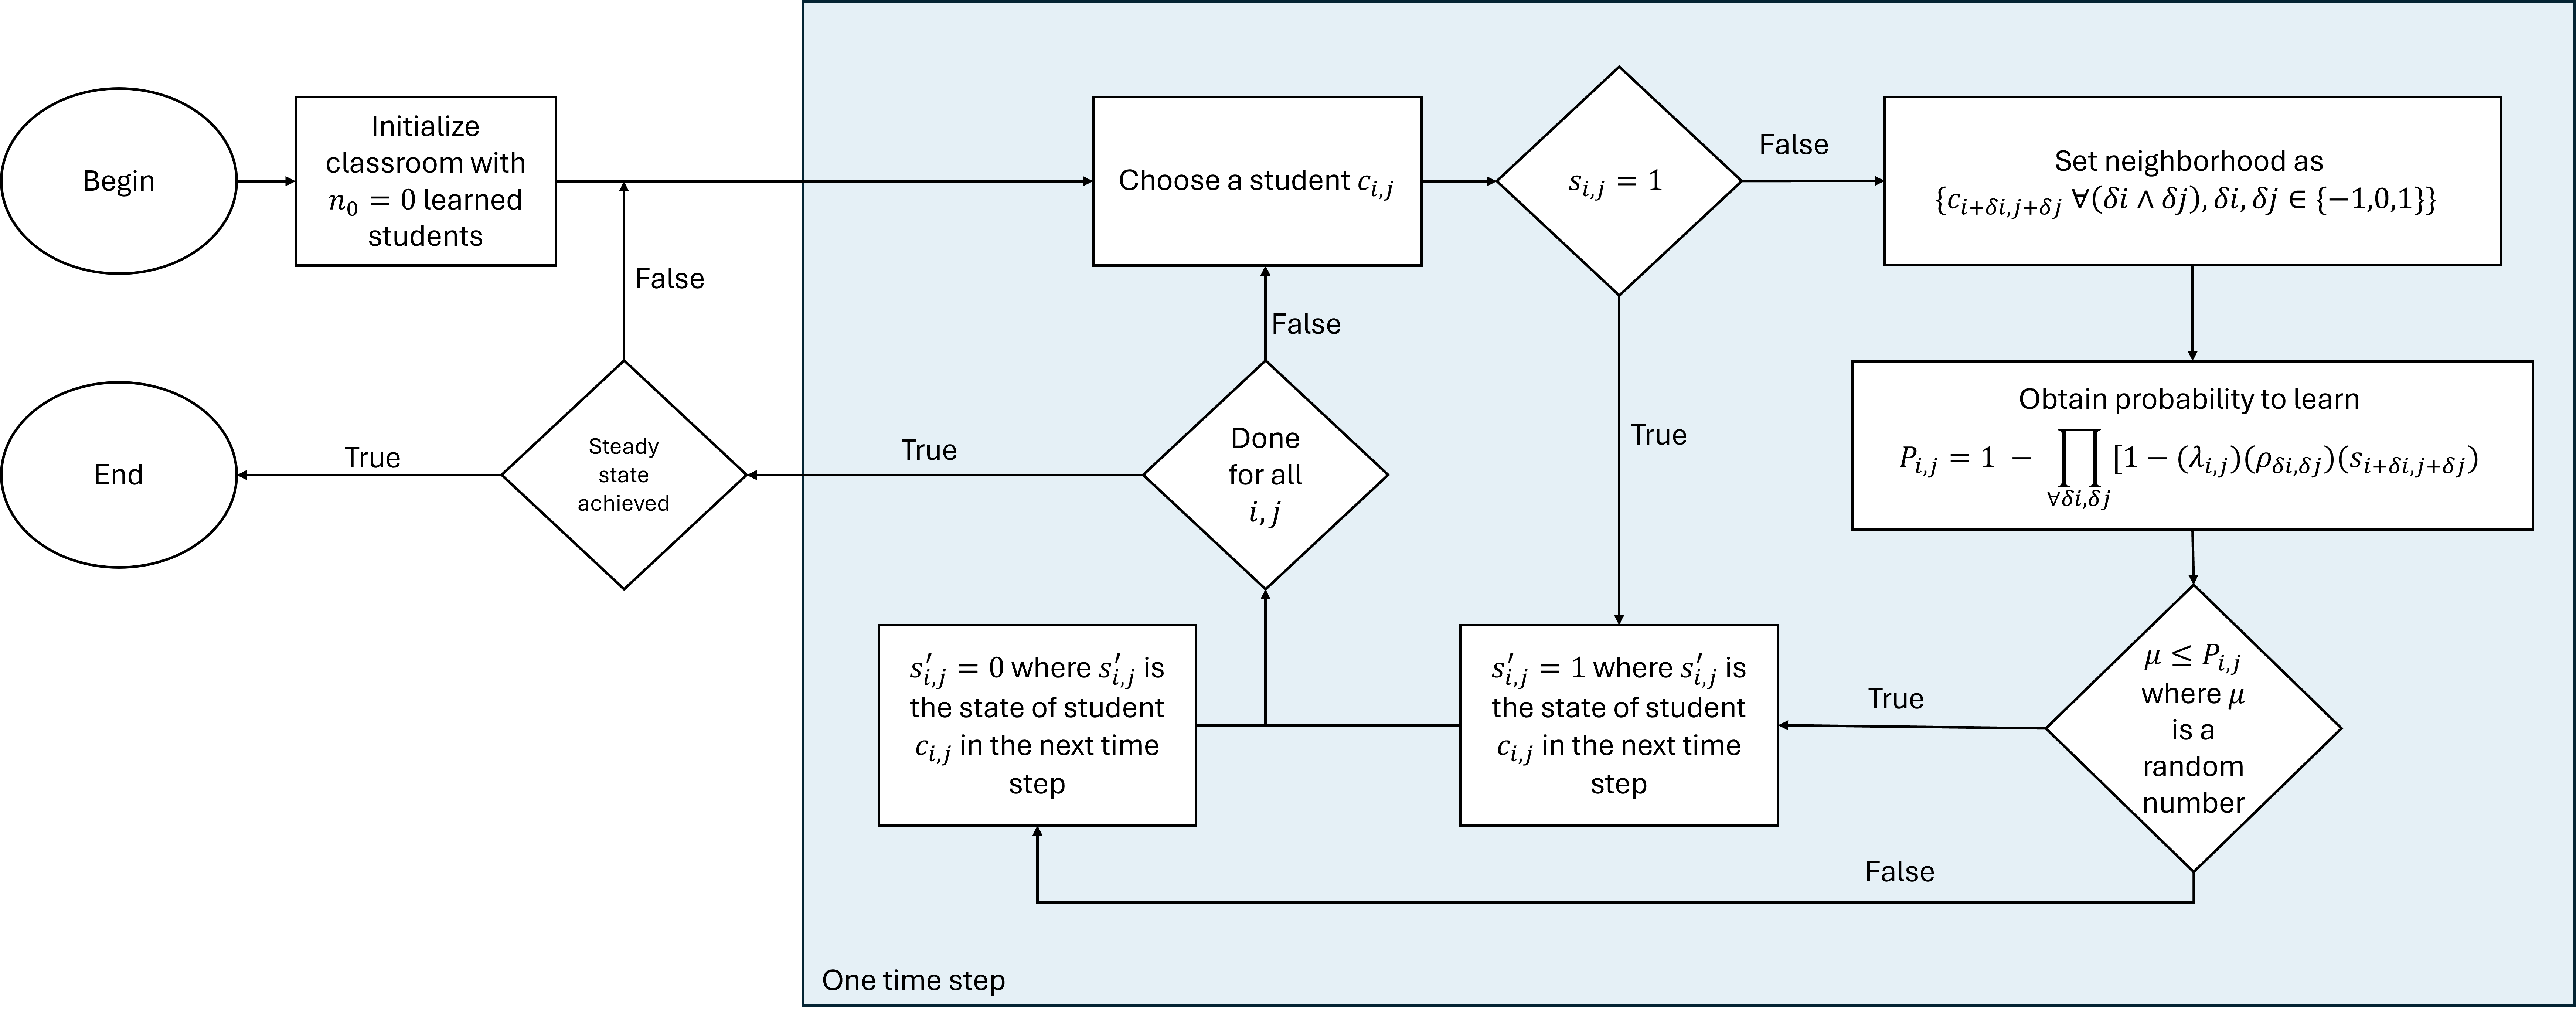
\includegraphics[width=0.45\textwidth]{figures/2DBPCA PI Flowchart.png}
            \caption[Peer instruction simulation flowchart]{Numerical process for simulation of 2D BPCA for peer instruction.}
            \label{fig:PI flowchart}
        \end{figure}


    \subsection{Model parameters}
        The values of the model input parameters we considered for the class size $N=L^2$, the positional learning coefficient $\rho_0$, and the learning rate heterogeneity $\delta\lambda$ are as follows:

        \begin{itemize}
            \item $L=\lbrace32,48,64,96,128\rbrace$
            \item $\rho_0=\lbrace0.1, 0.2, 0.3,\dots, 0.8, 0.9, 1.0\rbrace$
            \item $\delta\lambda=\lbrace0.0, 0.1, 0.2, 0.3, 0.4\rbrace$
        \end{itemize}

        To assess how well the class performed, we used the time it took for all the students to learn $t_{max}$.
        For both TI and PI, the simulation ends when all students have learned.
        Each set of parameters was run 5 independent times to get the average and standard deviation of $t_{max}$ for each set of parameters.


        %! Further investigation:
        %! When comparing learning rate of TI vs PI, TI is lower - wrong based on observation. The way we obtained learning rate m does not capture the two-stage learning process of TI. Will omit on this paper because I don't know how to fix that.
        %! TLDR: obtaining m leads to some kind of sampling error. Not the first time.

        % The class's average learning rate $m$ was calculated by taking the fraction of learned students as a function of time then fitting a power law ($y=ax^m$) to a fraction of the data using the Levenberg-Marquardt algorithm.
        % We chose to fit the power law only to the first half or quarter of the data for peer instruction and traditional instruction respectively so that we obtain the class learning rate before the finite size effect become significant.

\section{Results and Discussion}

    \subsection{Different Dynamics of Traditional and Peer Instruction}
        
        When we vary class size $N$, as shown in Figure~\ref{fig:comparison size}, we see that in TI remains constant with only time to learn $t_{max}$ increasing with class size $N$.
        For PI, increasing class size $N$ adds a time delay to when the learning starts to speed up. Despite the added time delay, the shape of the learning curve remains the same.
        The increase in time to learn $t_{max}$ is also less pronounced in PI compared to TI.

        \begin{figure}[htbp!]
            \centering
            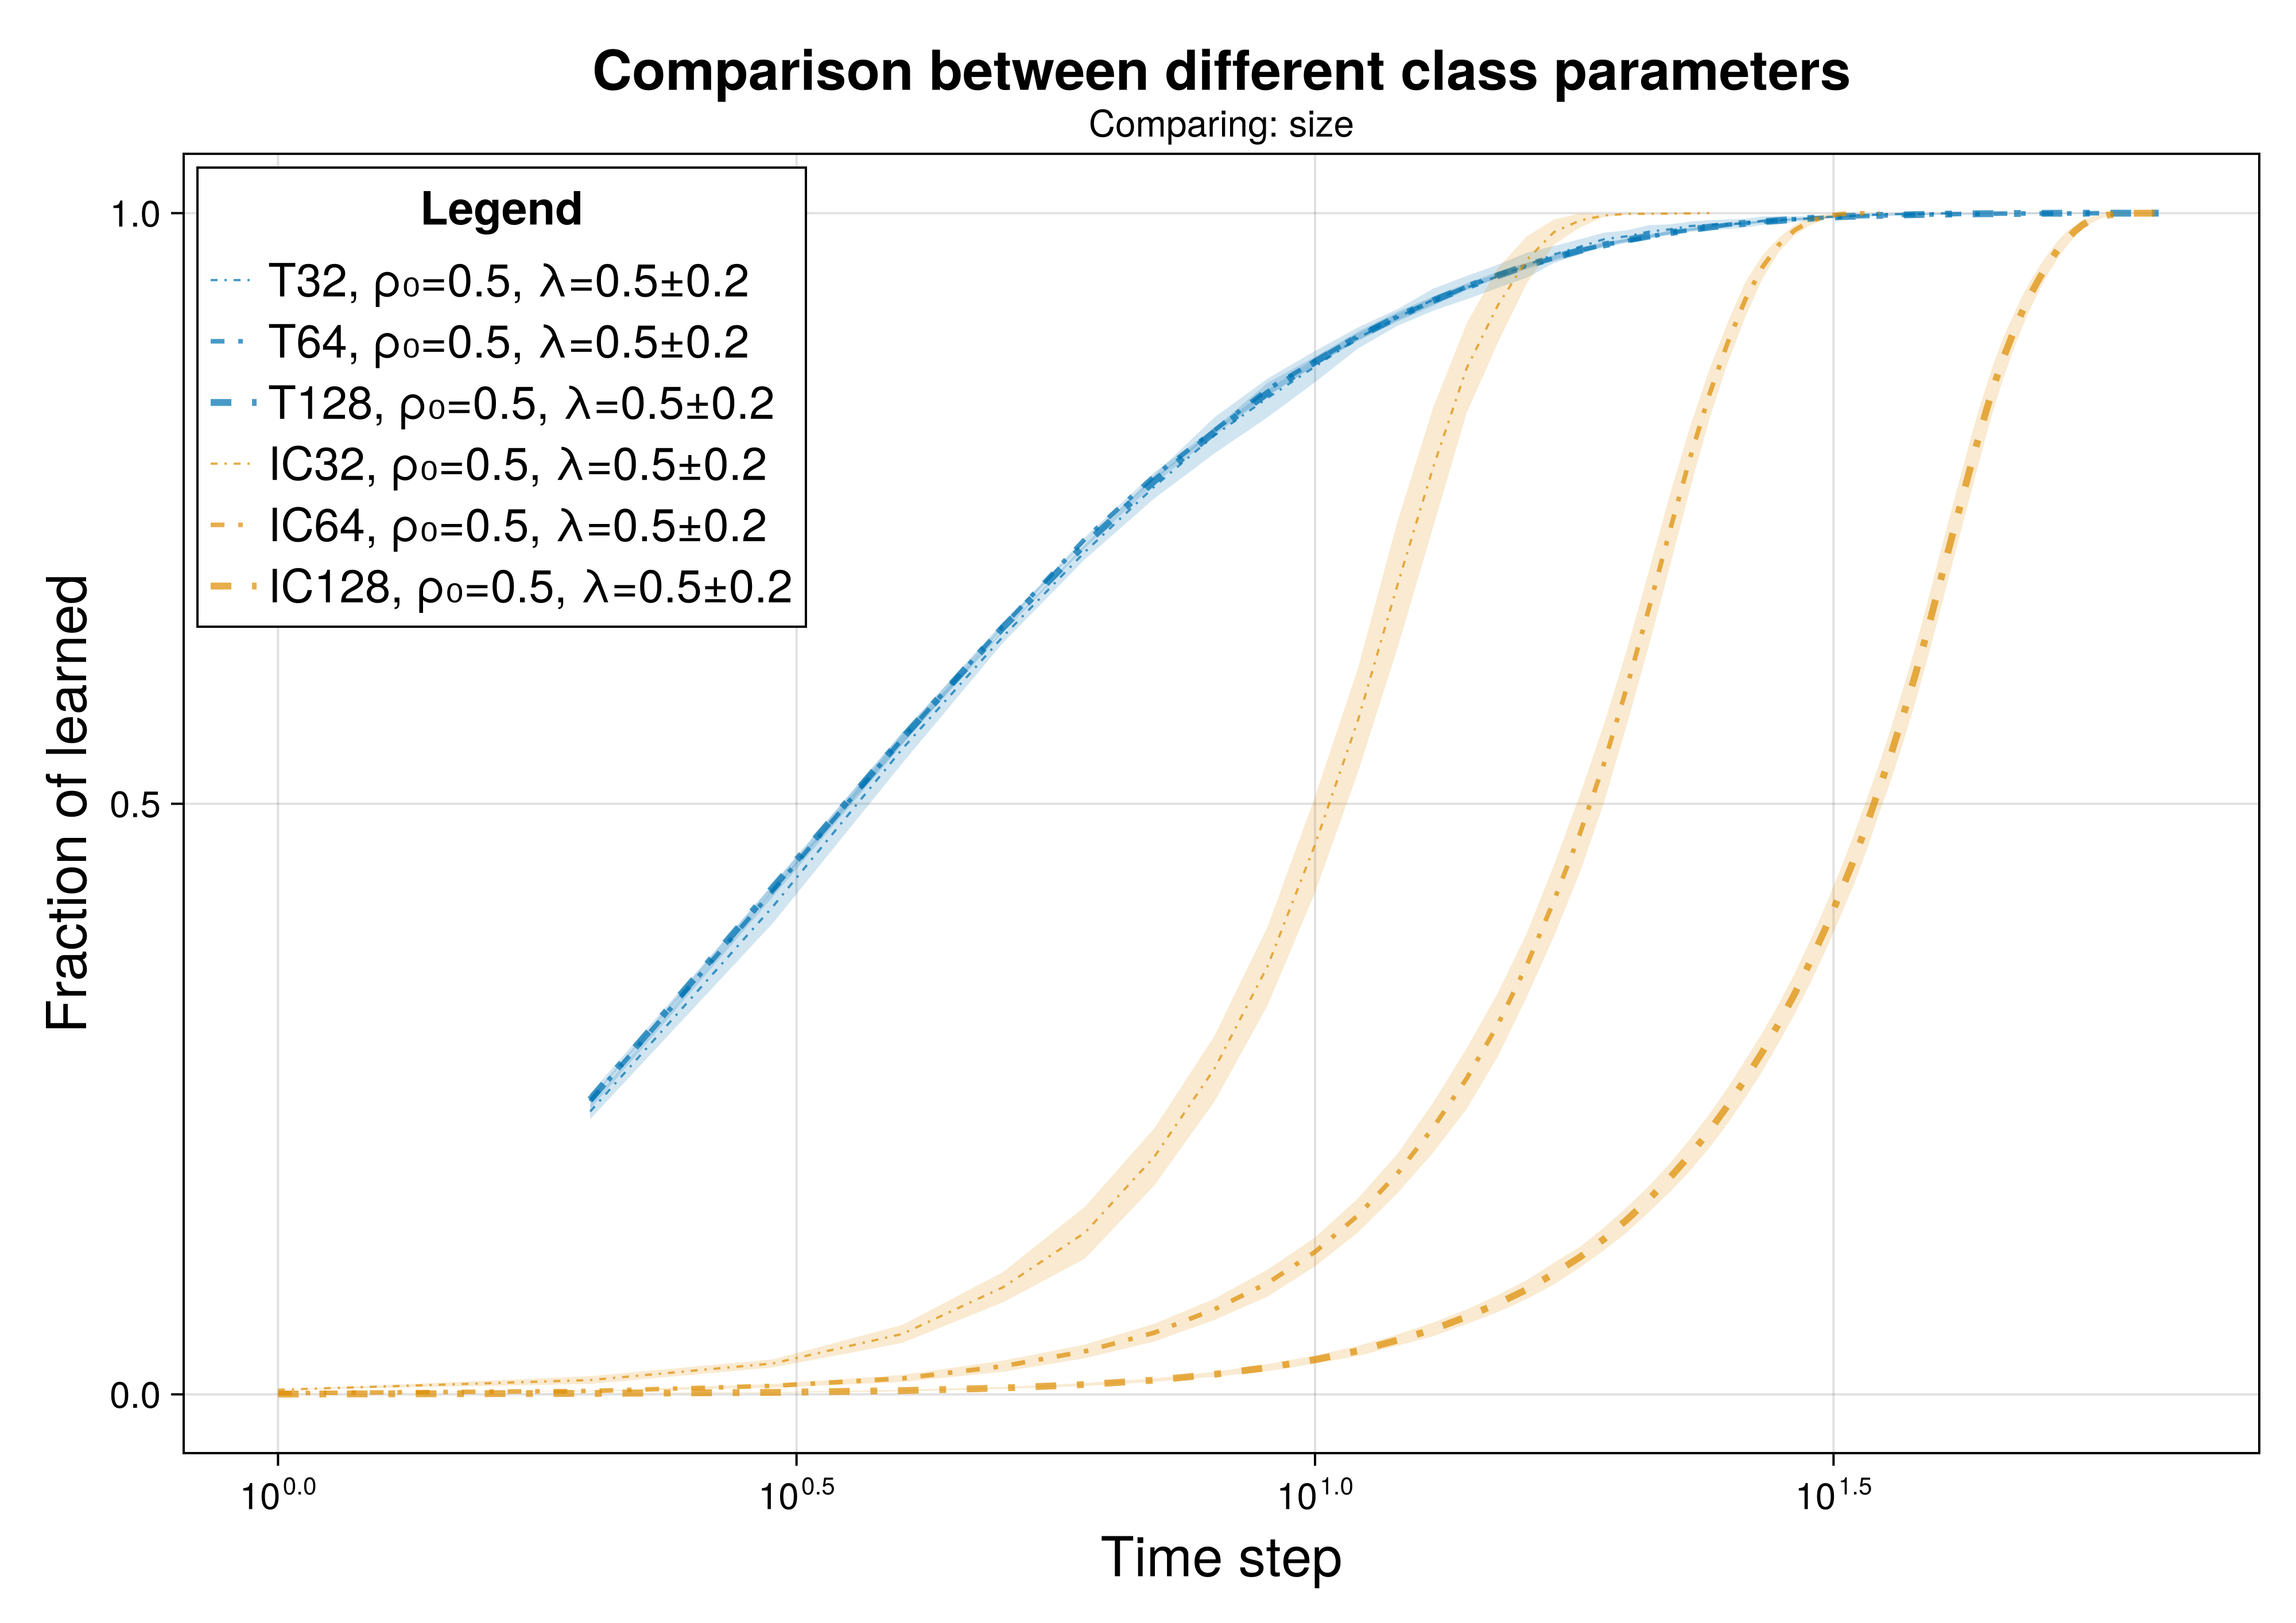
\includegraphics[width=0.45\textwidth]{figures/2D-BPCAIH-analysis/comparison plots/size.png}
            \caption{Comparison of time to learn $t_{max}$ and fraction of learned students for class size $N$.
            Each SA corresponds to a different color --- blue for traditional, orange for inner corner.
            Different class sizes correspond to different line widths where bigger classroom sizes are represented by thicker lines.
            The bands around each line show the standard deviation of the daya over 5 trials.
            Higher fraction of learned students indicate better learning.}
            \label{fig:comparison size}
        \end{figure}

        Varying positional learning factor $\rho_0$, shown in Figure~\ref{fig:comparison ρ₀}, varies the shape of the learning curve for TI, especially for lower values of positional learning factor $\rho_0$.
        For traditional instruction, changes in $\rho_0$ affects the number of students that learn in the second time step and the rate of which students learn throughout the class.
        For peer instruction, the shape of the learning curve remains the same for different values of $\rho_0$, only adding a time delay to when the learning starts to speed up --- similar to the effects of class size $N$.
        Additionally, the effect of varying positional learning factor $\rho_0$ is nonlinear for both models. Those with extremely low values of $\rho_0$, like those of $\rho_0=0.1$, perform much worse with learning curves being further from $\rho_0=0.5$ than $\rho_0=0.9$ is with $\rho_0=0.5$.

        \begin{figure}[htbp!]
            \centering
            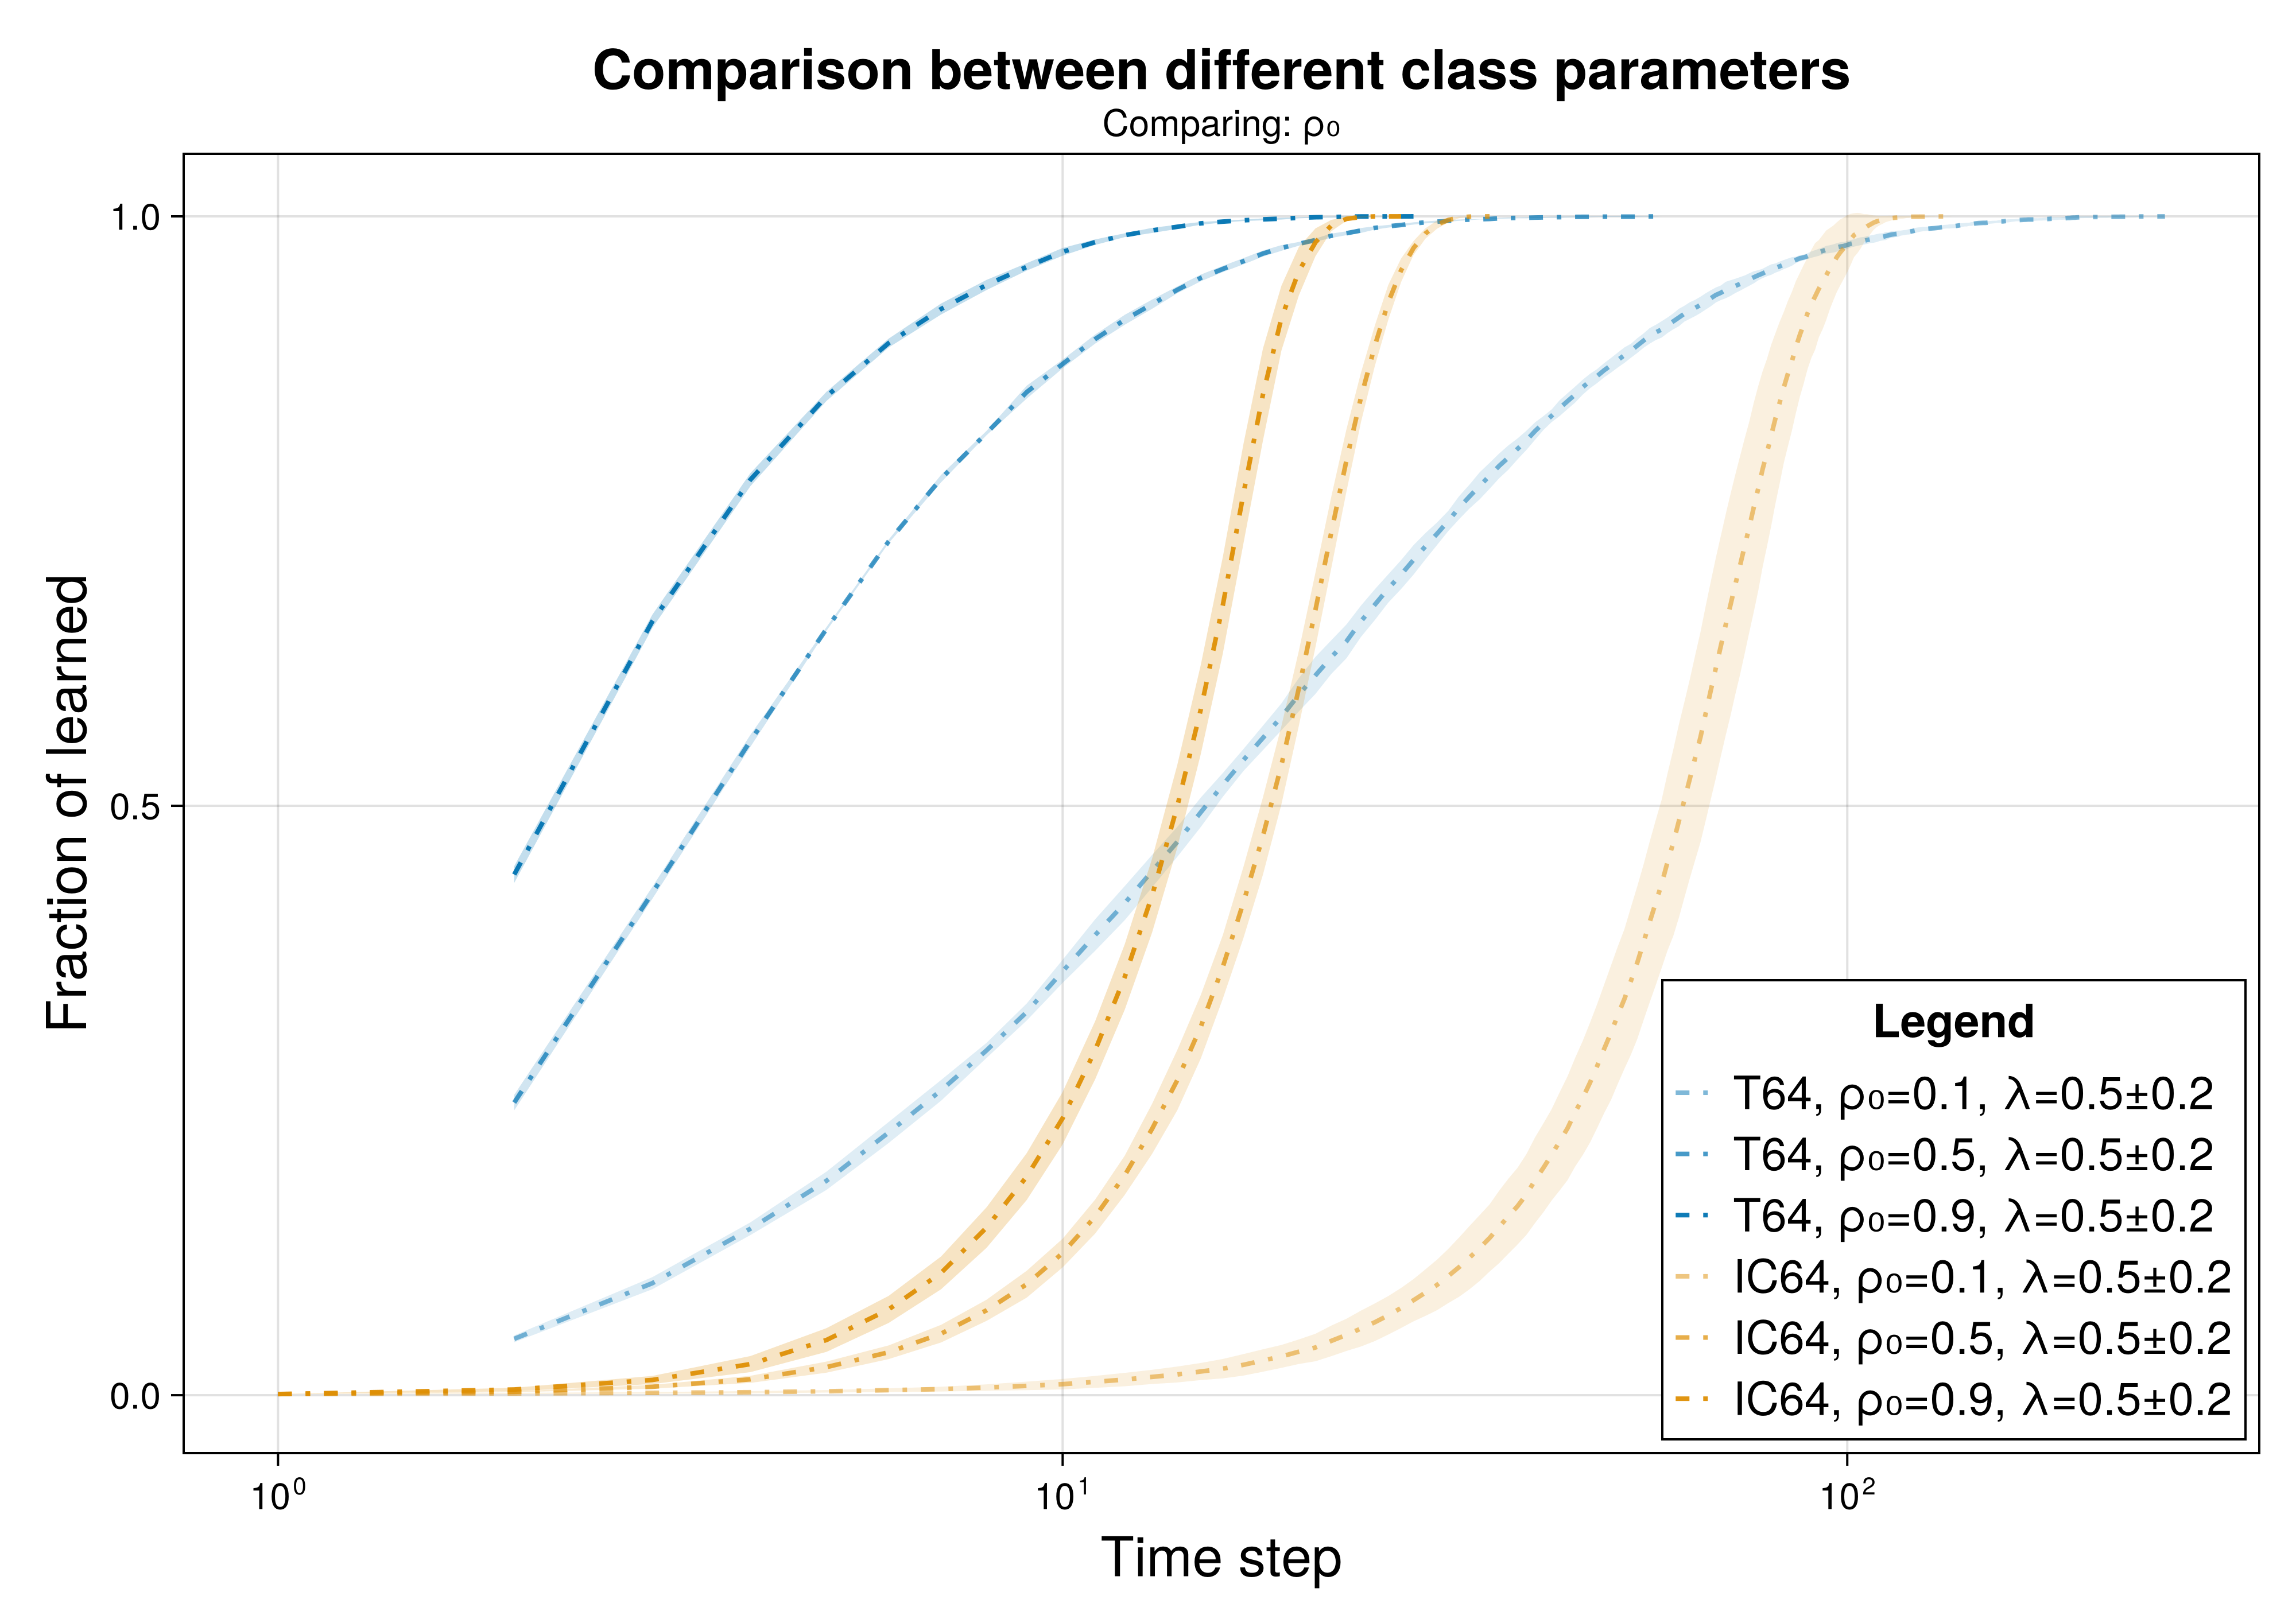
\includegraphics[width=0.45\textwidth]{figures/2D-BPCAIH-analysis/comparison plots/ρ₀.png}
            \caption{Comparison of time to learn $t_{max}$ and fraction of learned students for positional learning factor $\rho_0$.
            Each SA corresponds to a different color --- blue for traditional, orange for inner corner.
            Different $\rho_0$ values correspond to different line transparancies where darker lines represent higher $\rho_0$ values.
            The bands around each line show the standard deviation of the daya over 5 trials.
            Higher fraction of learned students indicate better learning.}
            \label{fig:comparison ρ₀}
        \end{figure}

        Figure~\ref{fig:comparison δλ} shows that an increase in heterogeneity $\delta\lambda$ changes how fast the slope of the learning curve changes for TI without changing the initial number of learned students.
        For PI, only very high values of heterogeneity $\delta\lambda$ noticeably affect the learning curve.
        As with the positional learning factor $\rho_0$, the effect of varying heterogeneity $\delta\lambda$ is similar to that of class size $N$ --- only adding a time delay to when the learning starts to speed up.

        \begin{figure}[htbp!]
            \centering
            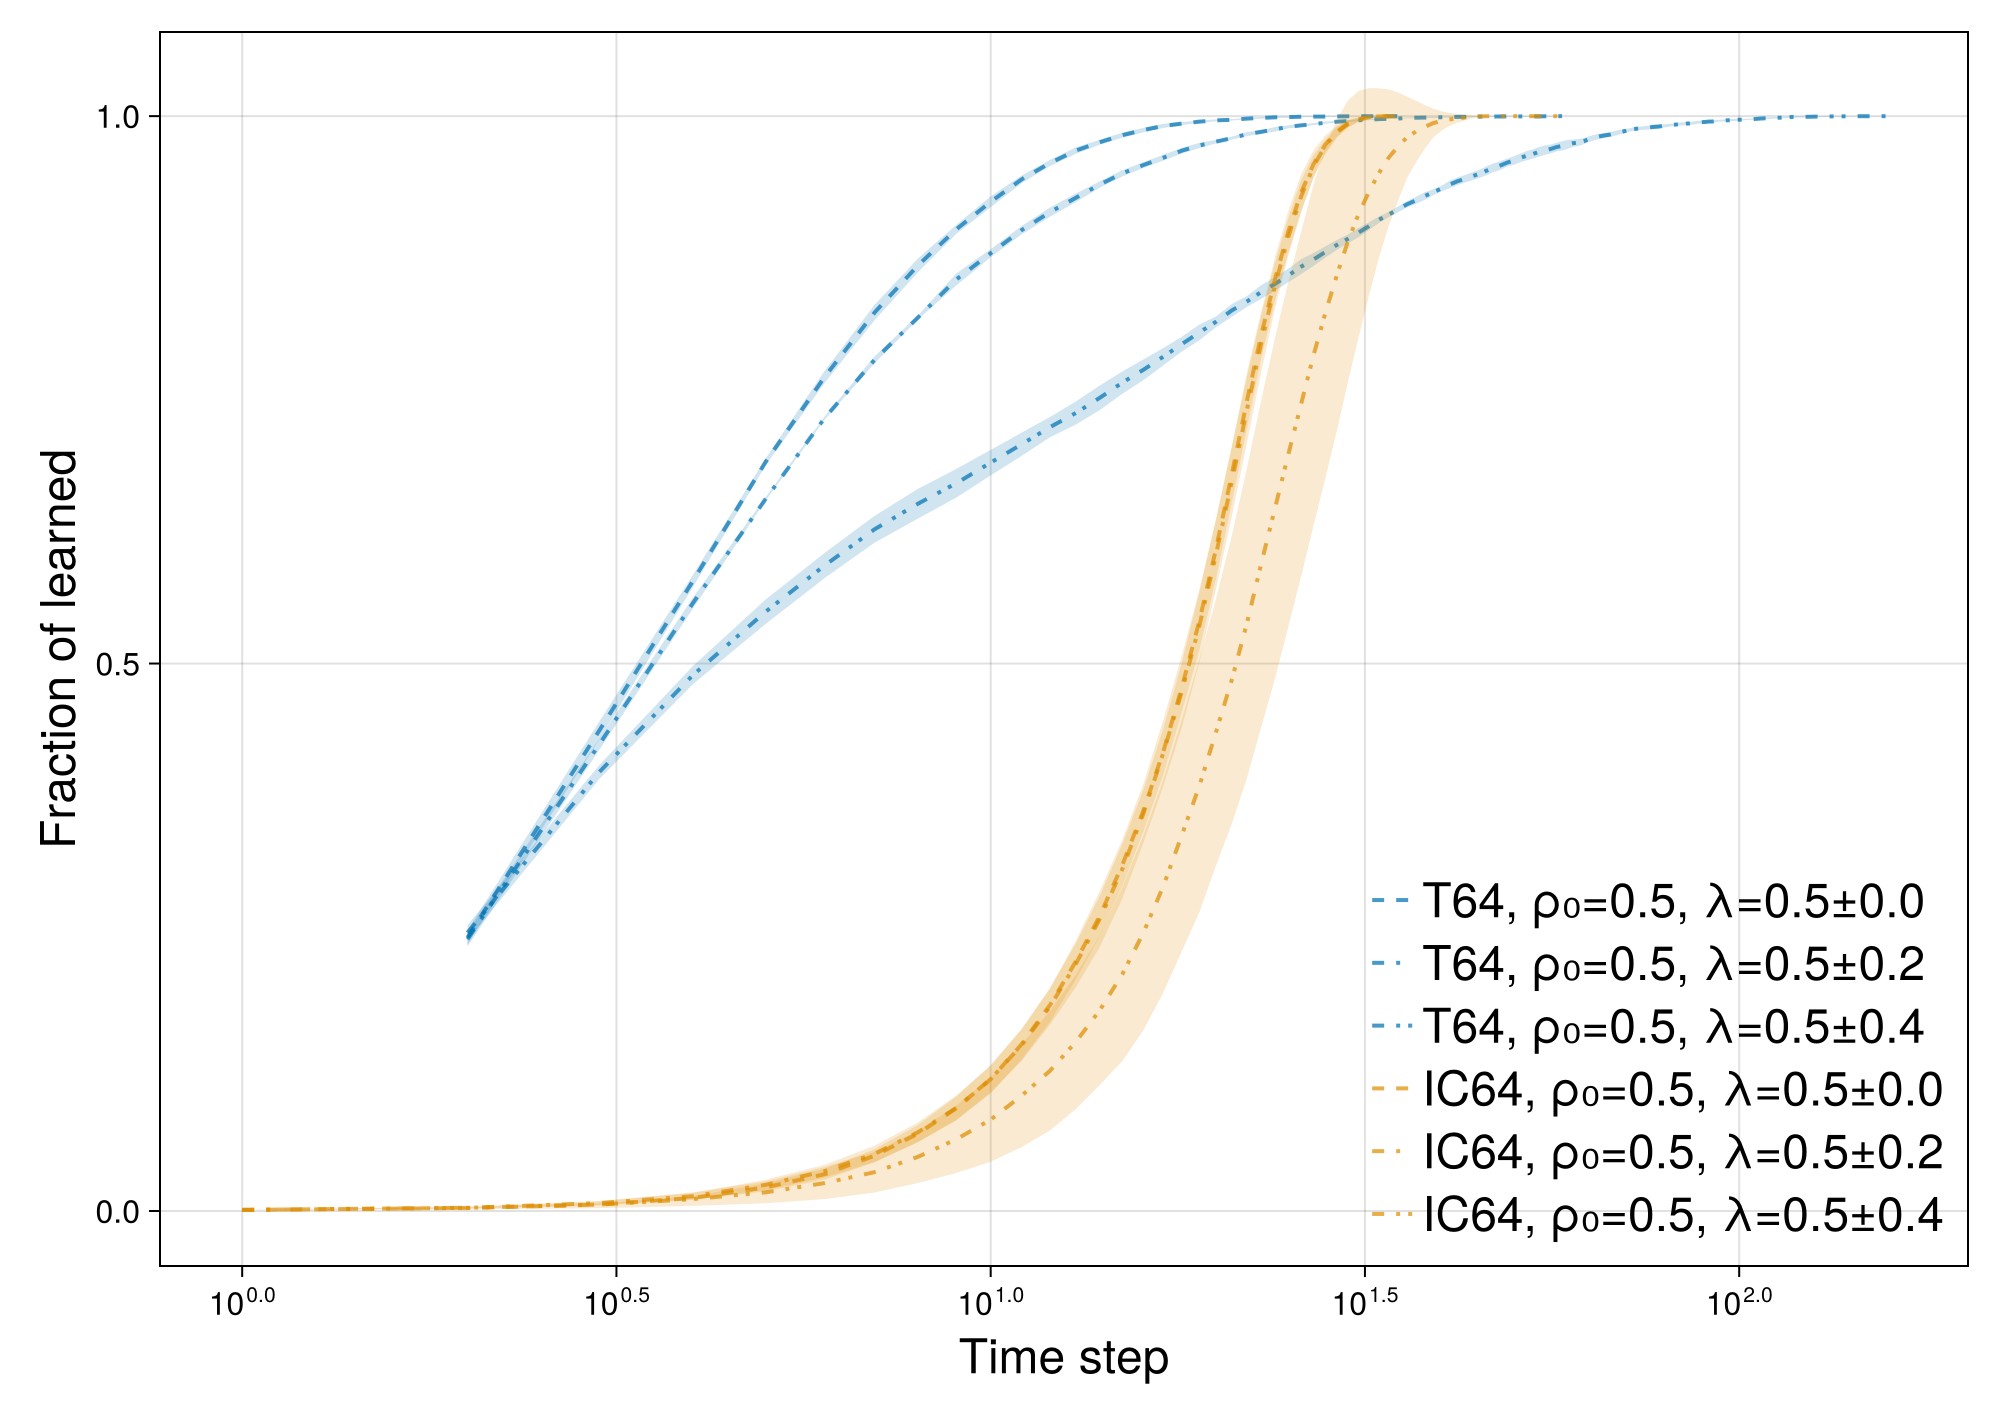
\includegraphics[width=0.45\textwidth]{figures/2D-BPCAIH-analysis/comparison plots/δλ.png}
            \caption{Comparison of time to learn $t_{max}$ and fraction of learned students for different learning rate heterogeneity $\delta\lambda$.
            Each SA corresponds to a different color --- blue for traditional, orange for inner corner.
            Different $\delta\lambda$ values correspond to different line styles where $\delta\lambda=0,0.2,0.4$ are represented by dashed lines, alternating dots and dashes, and two dots and a dash respectively.
            The bands around each line show the standard deviation of the daya over 5 trials.
            Higher fraction of learned students indicate better learning.}
            \label{fig:comparison δλ}
        \end{figure}

        We also investigate the effects of seating arrangement for PI in Figure~\ref{fig:comparison SA}.
        For the set of parameters $L=64,\space\rho_0=0.5,\space\delta\lambda=0.2$, we find that the inner corner seating arrangement performs the best in terms of both the time it takes for all the students to learn and the classroom's learning rate.
        Furthermore, we see that TI performs better than PI, especially for the earlier time steps.

        \begin{figure}[htbp!]
            \centering
            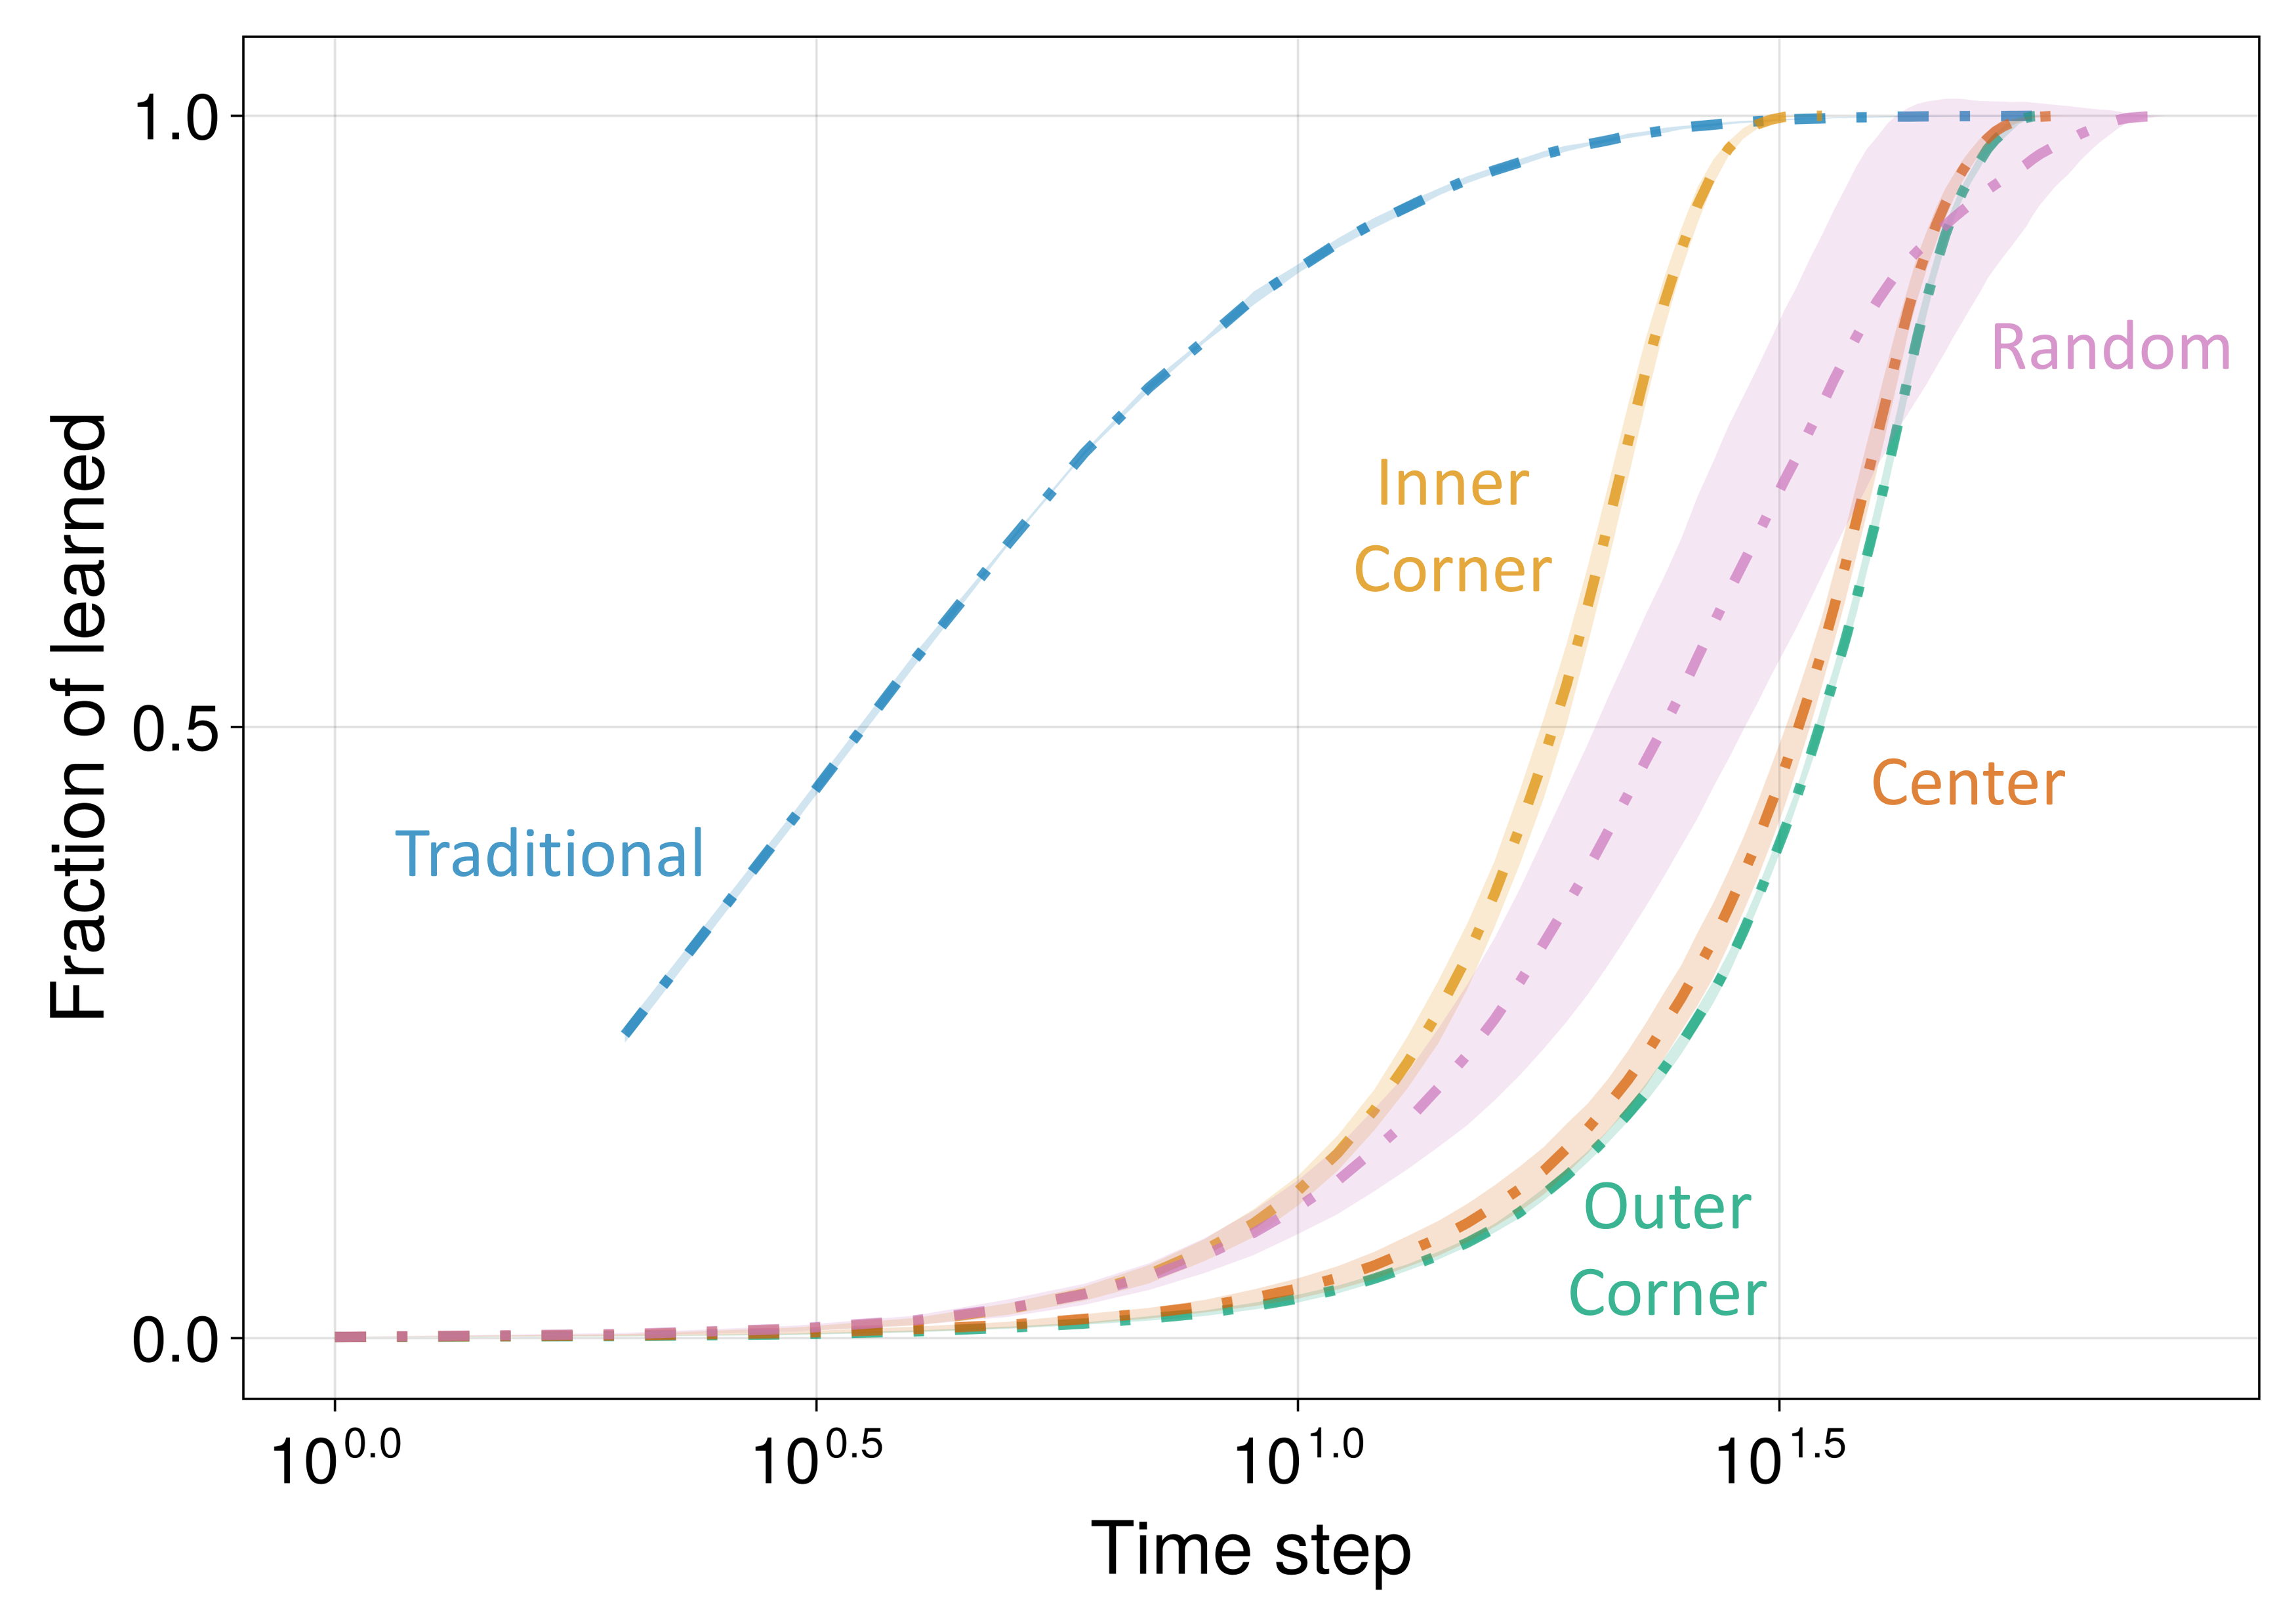
\includegraphics[width=0.45\textwidth]{figures/2D-BPCAIH-analysis/comparison plots/SA.png}
            \caption{Comparison of time to learn $t_{max}$ and fraction of learned students for different SAs.
            Each SA corresponds to a different color --- blue for traditional, orange for inner corner, green for outer corner, orange for center, and pink for random.
            The bands around each line show the standard deviation of the daya over 5 trials.
            Higher fraction of learned students indicate better learning.}
            \label{fig:comparison SA}
        \end{figure}

        From all the plots shown in this section, we can also observe that TI has more students learning in the earlier time steps, but has lower time to learn $t_{max}$ when compared to PI for the same set of parameters.
        This suggests that when performing TI, more time is spent waiting for slower learners than when performing PI.

        Investigating this phenomenon further, we find that the learning curve for TI has two stages: a fast initial stage and a slow final stage.
        The fast initial stage is characterized by a sharp increase in the number of learned students, this is caused by the majority of fast students learning quickly.
        The slow stage is characterized by a much slower increase in the number of learned students, this is caused by waiting for the slower students to learn.
        This phenomenon is seen in Figure~\ref{fig:comparison δλ} where the TI case where the students have a homogenous learning rate ($\delta\lambda=0$) show a consistent slope throughout the simulation compared to cases with heterogeneity ($\delta\lambda>0$) where the two-stage learning process is more evident.

        This hypothesis is further supported when investigating specific cases where the two-stage learning process is expected to be more pronounced --- classes under TI with low positional learning factor $\rho_0$ and high learning rate heterogeneity $\delta\lambda$.
        Figure~\ref{fig:two stage learning} shows one trial of a class under TI with $L=64$, $\rho_0=0.3$, and $\delta\lambda=0.4$.
        We see that for $t=2$, the majority of the student that learned are those with higher learning rates ($\lambda=0.5+0.4$).
        By $t=13$, the slower students have started to learn, but the rate of learning has slowed down significantly as the majority of students with higher learning rate have already learned.
        This simulation will spend up to $t=232$ waiting for the slower students to learn.

    \begin{figure}[htbp!]
        \centering
        \subfigure[$t=2$]{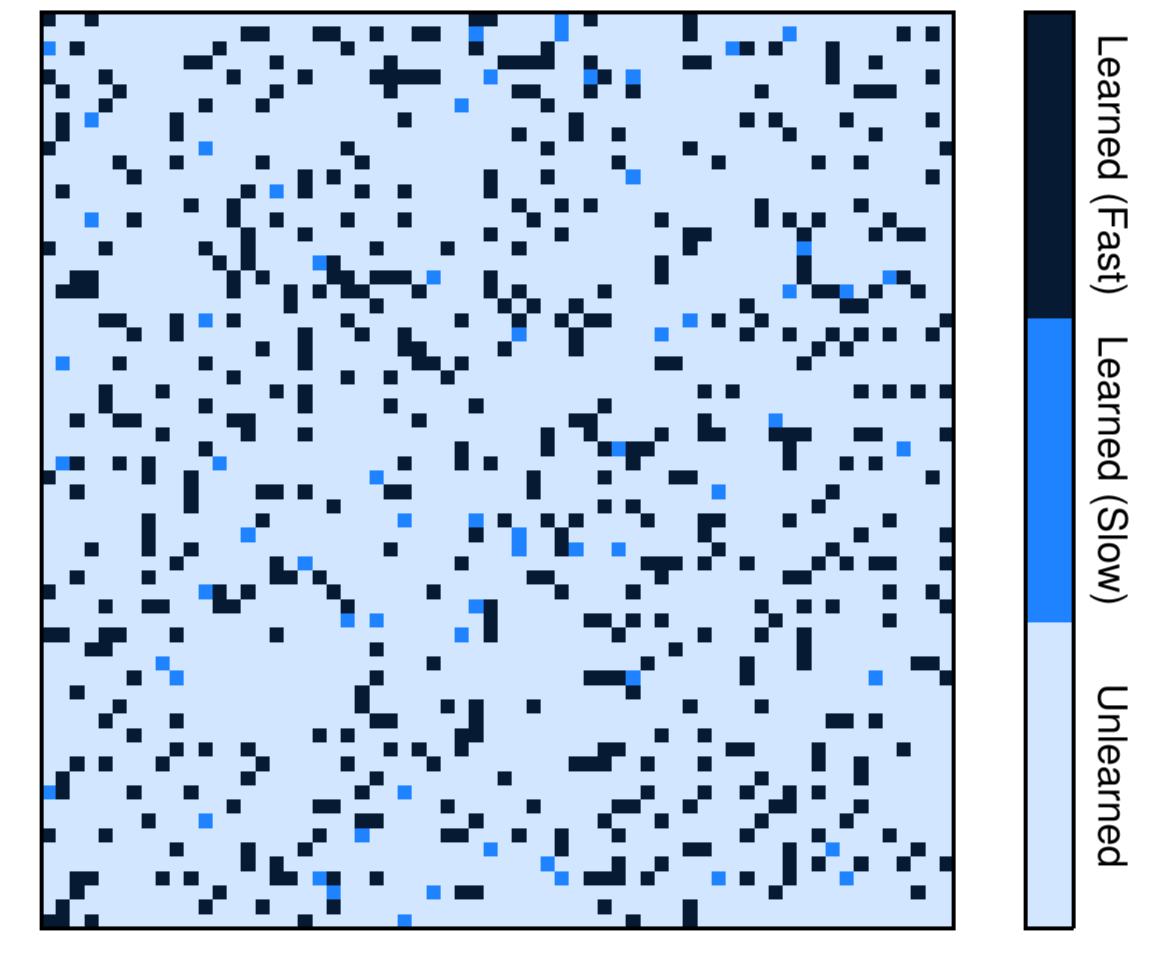
\includegraphics[width=0.23\textwidth]{figures/2D-BPCAIH-analysis/class evolutions/trad low rho high delta/2DBPCAIH-traditional-64-0.3-0.5-0.4-trial_3-2.png}}
        \subfigure[$t=13$]{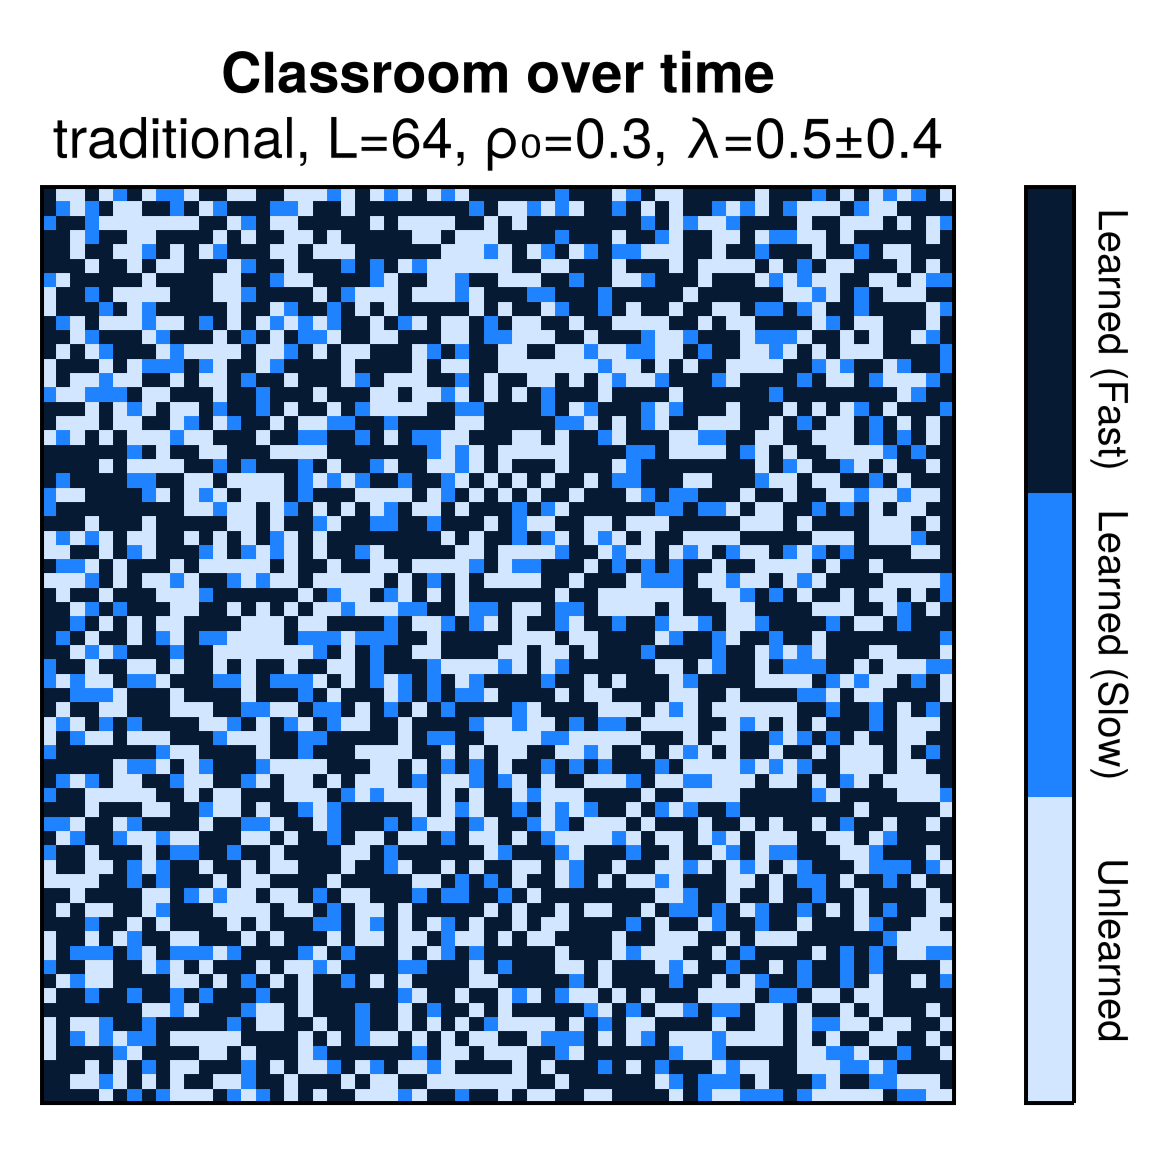
\includegraphics[width=0.23\textwidth]{figures/2D-BPCAIH-analysis/class evolutions/trad low rho high delta/2DBPCAIH-traditional-64-0.3-0.5-0.4-trial_3-13.png}}
        \caption{Example classroom evolution for TI with $L=64$, $\rho_0=0.3$, and $\delta\lambda=0.4$ at different time steps $t$ showing a two-stage learning process.
        Dark blue cells represent learned students with learning rate $\lambda=\lambda_0+\delta\lambda$, blue cells represent learned students with learning rate $\lambda=\lambda_0-\delta\lambda$, and light blue cells represent unlearned students.}
        \label{fig:two stage learning}
    \end{figure}

    These findings suggests that to optimize the learning in the classroom, it would be best to perform TI at the start of the class to take advantage of the fast initial learning stage, then switch to PI where the time to learn $t_{max}$ is lower than TI for the same set of parameters.
    This is consistent with current practices as outlined by Mazur \cite{mazur1997peer} and modified by others \cite{smith2009peer,roxas2010seating,lasry2008peer}, where the students are expected to have read up on the material in advance and the instructor gives a short lecture before the students engage in peer discussion.

    \subsection{Summary of effects of class size $N$, positional learning factor $\rho_0$, and learning rate heterogeneity $\delta\lambda$}
        
        As we vary the different parameters, as shown in Figure~\ref{fig:Params effect summary t}, we are able to identify which cases are more favorable for TI or PI.
        We find that PI suffers more than TI when handling larger class sizes $N$, and that TI suffers more from increased learning rate heterogeneity $\delta\lambda$ compared to PI.
        However, low poisitonal learning factor $\rho_0$ affects both TI and PI similarly.

        The same figure also shows us the magnitude of the advantage of one method of instruction over the other.
        We find that when TI is advantageous, like in cases of big classrooms and low learning rate heterogeneity, the advantage over PI is not that large.
        However, in cases where PI is advantageous, like in cases of small classrooms and high learning rate heterogeneity, the advantage over TI is very large.
        This suggests that PI can be a safe option --- never performing much worse than TI, but can perform much better in certain cases.

        \begin{figure}[htbp!]
            \centering
            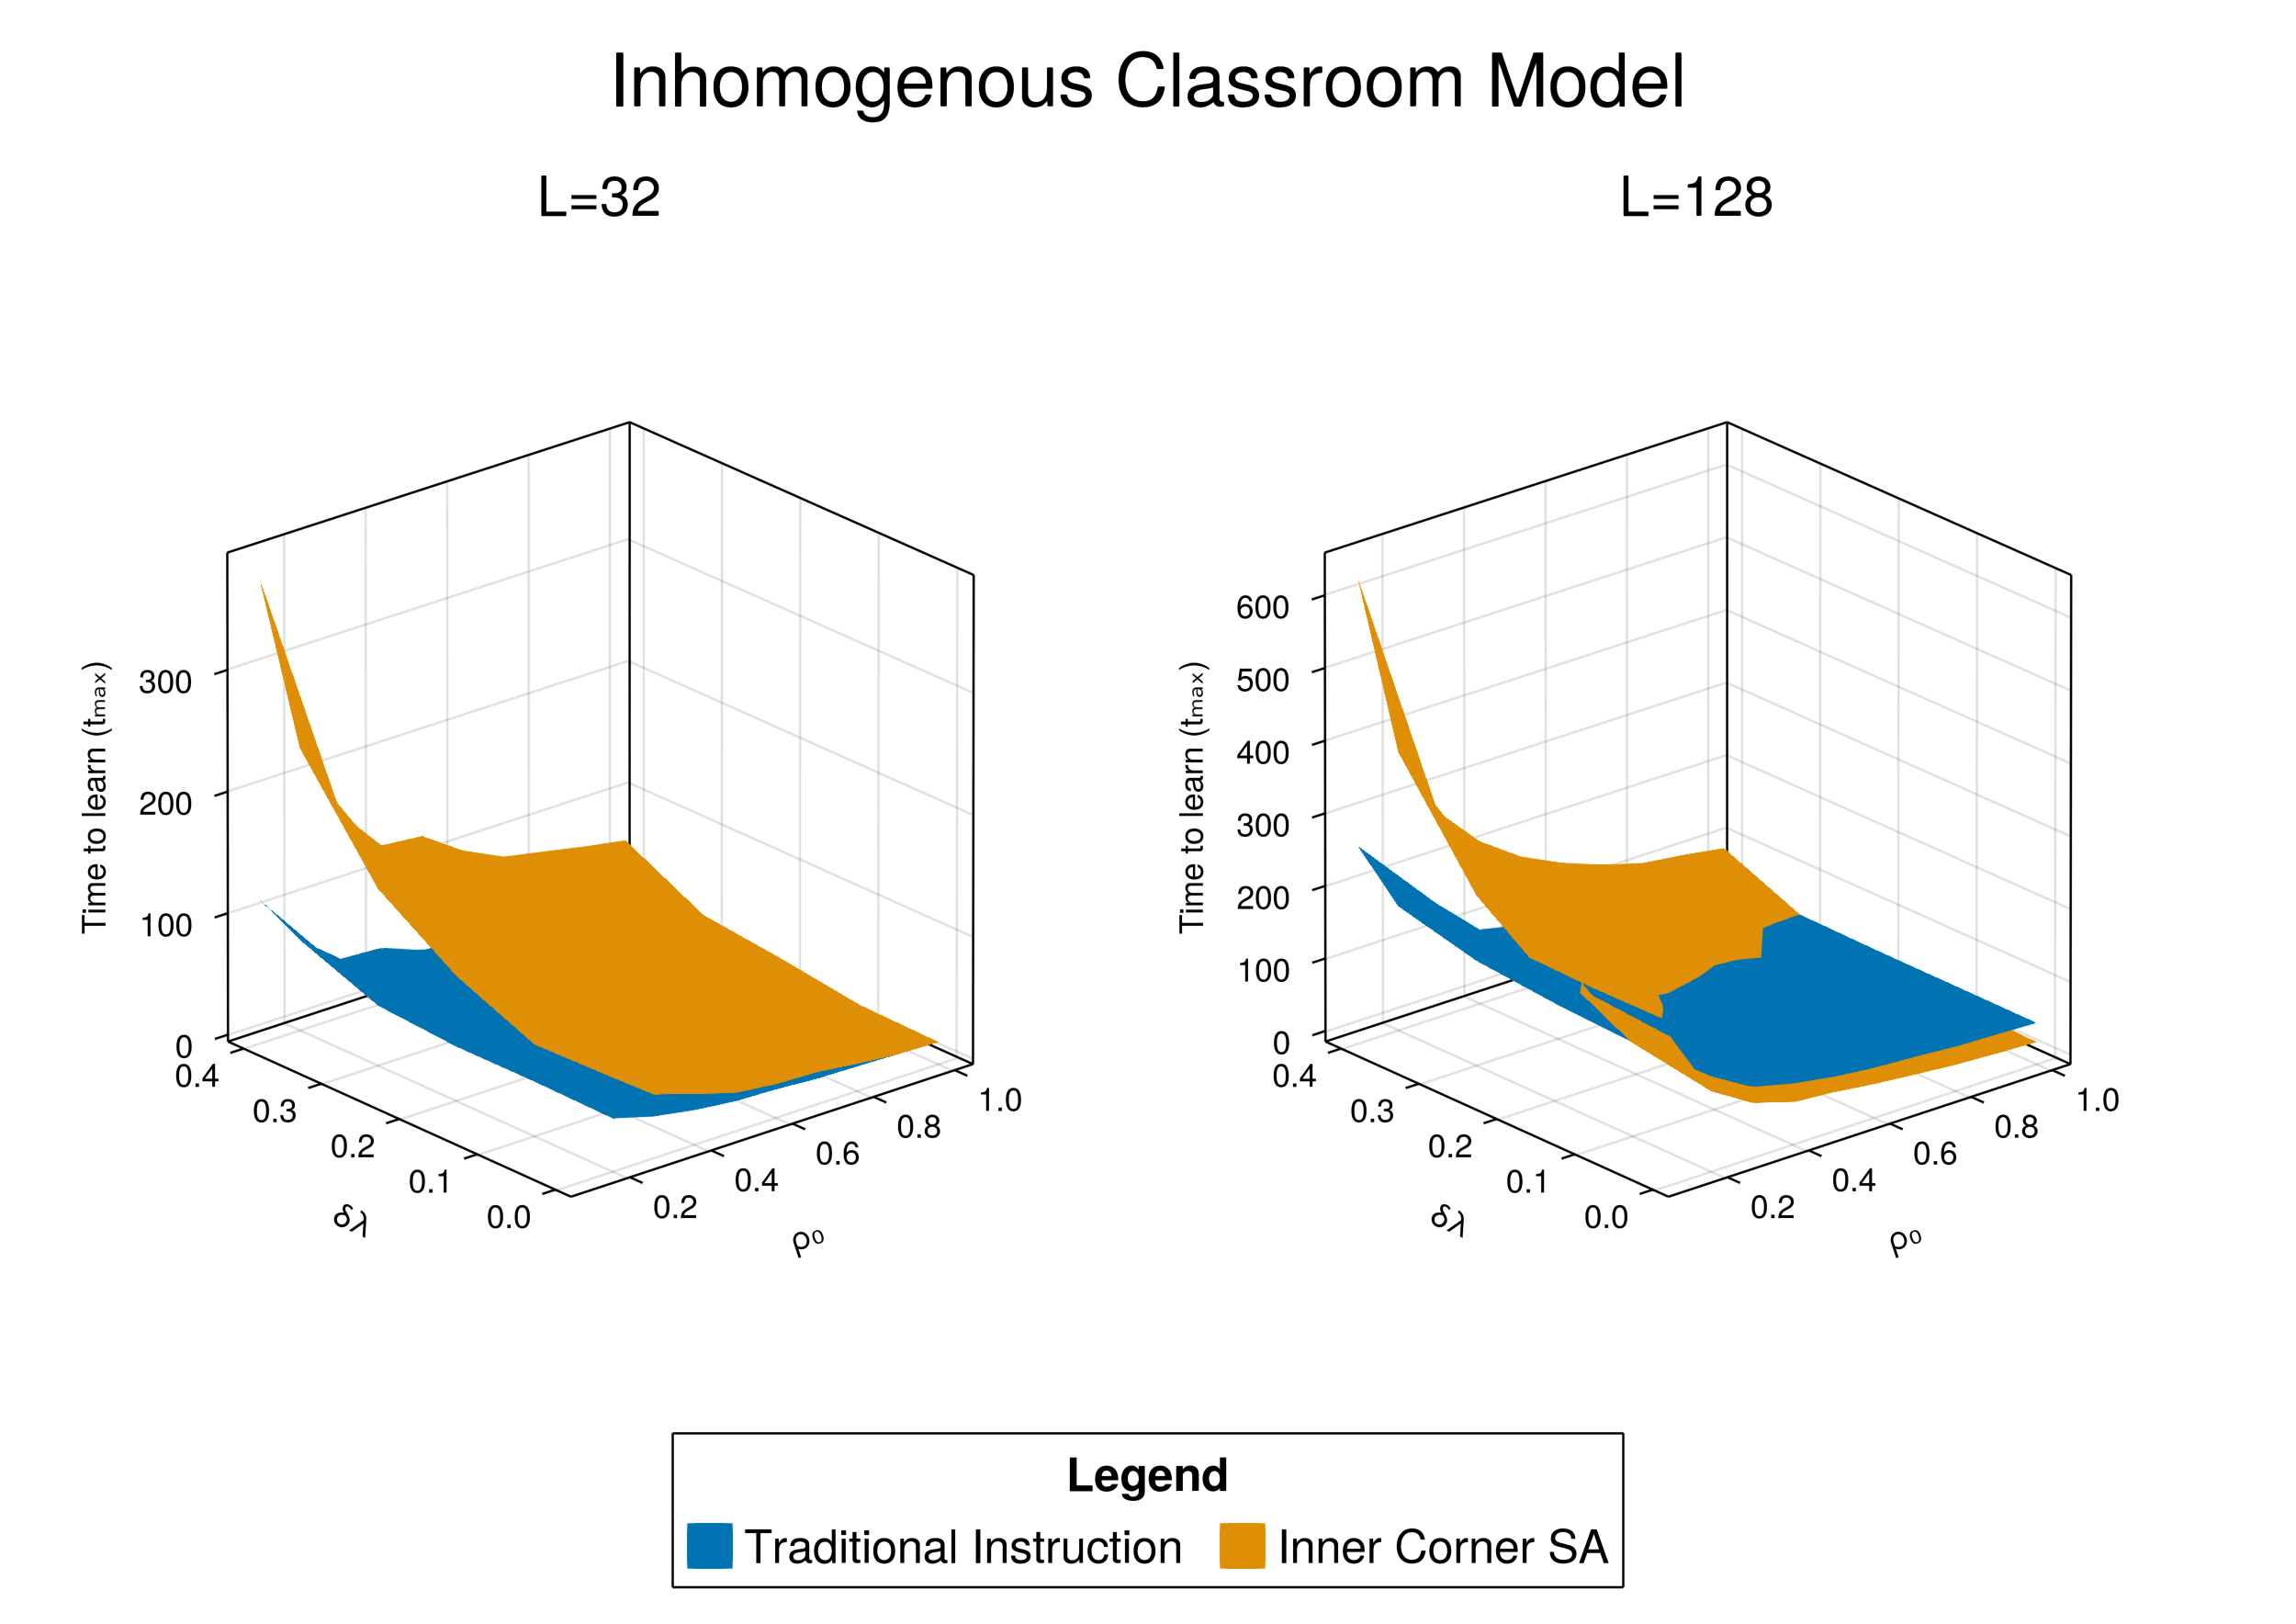
\includegraphics[width=0.47\textwidth]{figures/2D-BPCAIH-analysis/rho-dl-t plots/32-128 comparison.png}
            \caption{Time to learn $t_{max}$ as a function of positional learning factor $\rho_0$ and heterogeneity $\delta\lambda$ of PI (inner corner SA) and TI for different class sizes $N=L^2$.
            The blue surface represent TI and the orange surface represents PI.
            Lower time to learn indicates better learning.}
            \label{fig:Params effect summary t}
        \end{figure}

    \subsection{Comparison with existing research/data}
        
        Comparing our data to Nitta's model (Equation~\ref{eq: nitta model}) \cite{nitta2019mathematical}, as in Figure~\ref{fig:Return map}, only our data for PI approaches their model --- this is expected since their model is for PI and not TI.
        Furthermore, PI only approaches their model when the conditions are favorable for PI.
        Considering that their model has been shown to agree with experimental data, it suggests that real world students' behavior and learning dynamics are better represented by the values of high positional learning factor $\rho_0$ and small class sizes $N$.
        It should also be noted that Nitta's model and data tracks individual students' learning while our model tracks the class's learning as a whole.
        We chose to track learning this way because there is not much insight to be gained from tracking individual students' learning in a binary-state model.
        Nevertheless, the agreement of our model to theirs and to experimental data suggests that our model can be a good approximation of the real world with further improvements.

        \begin{figure}[htbp!]
            \centering
            \subfigure[$L=128,\space\rho_0=1,\space\lambda=0.5\pm0.4$]{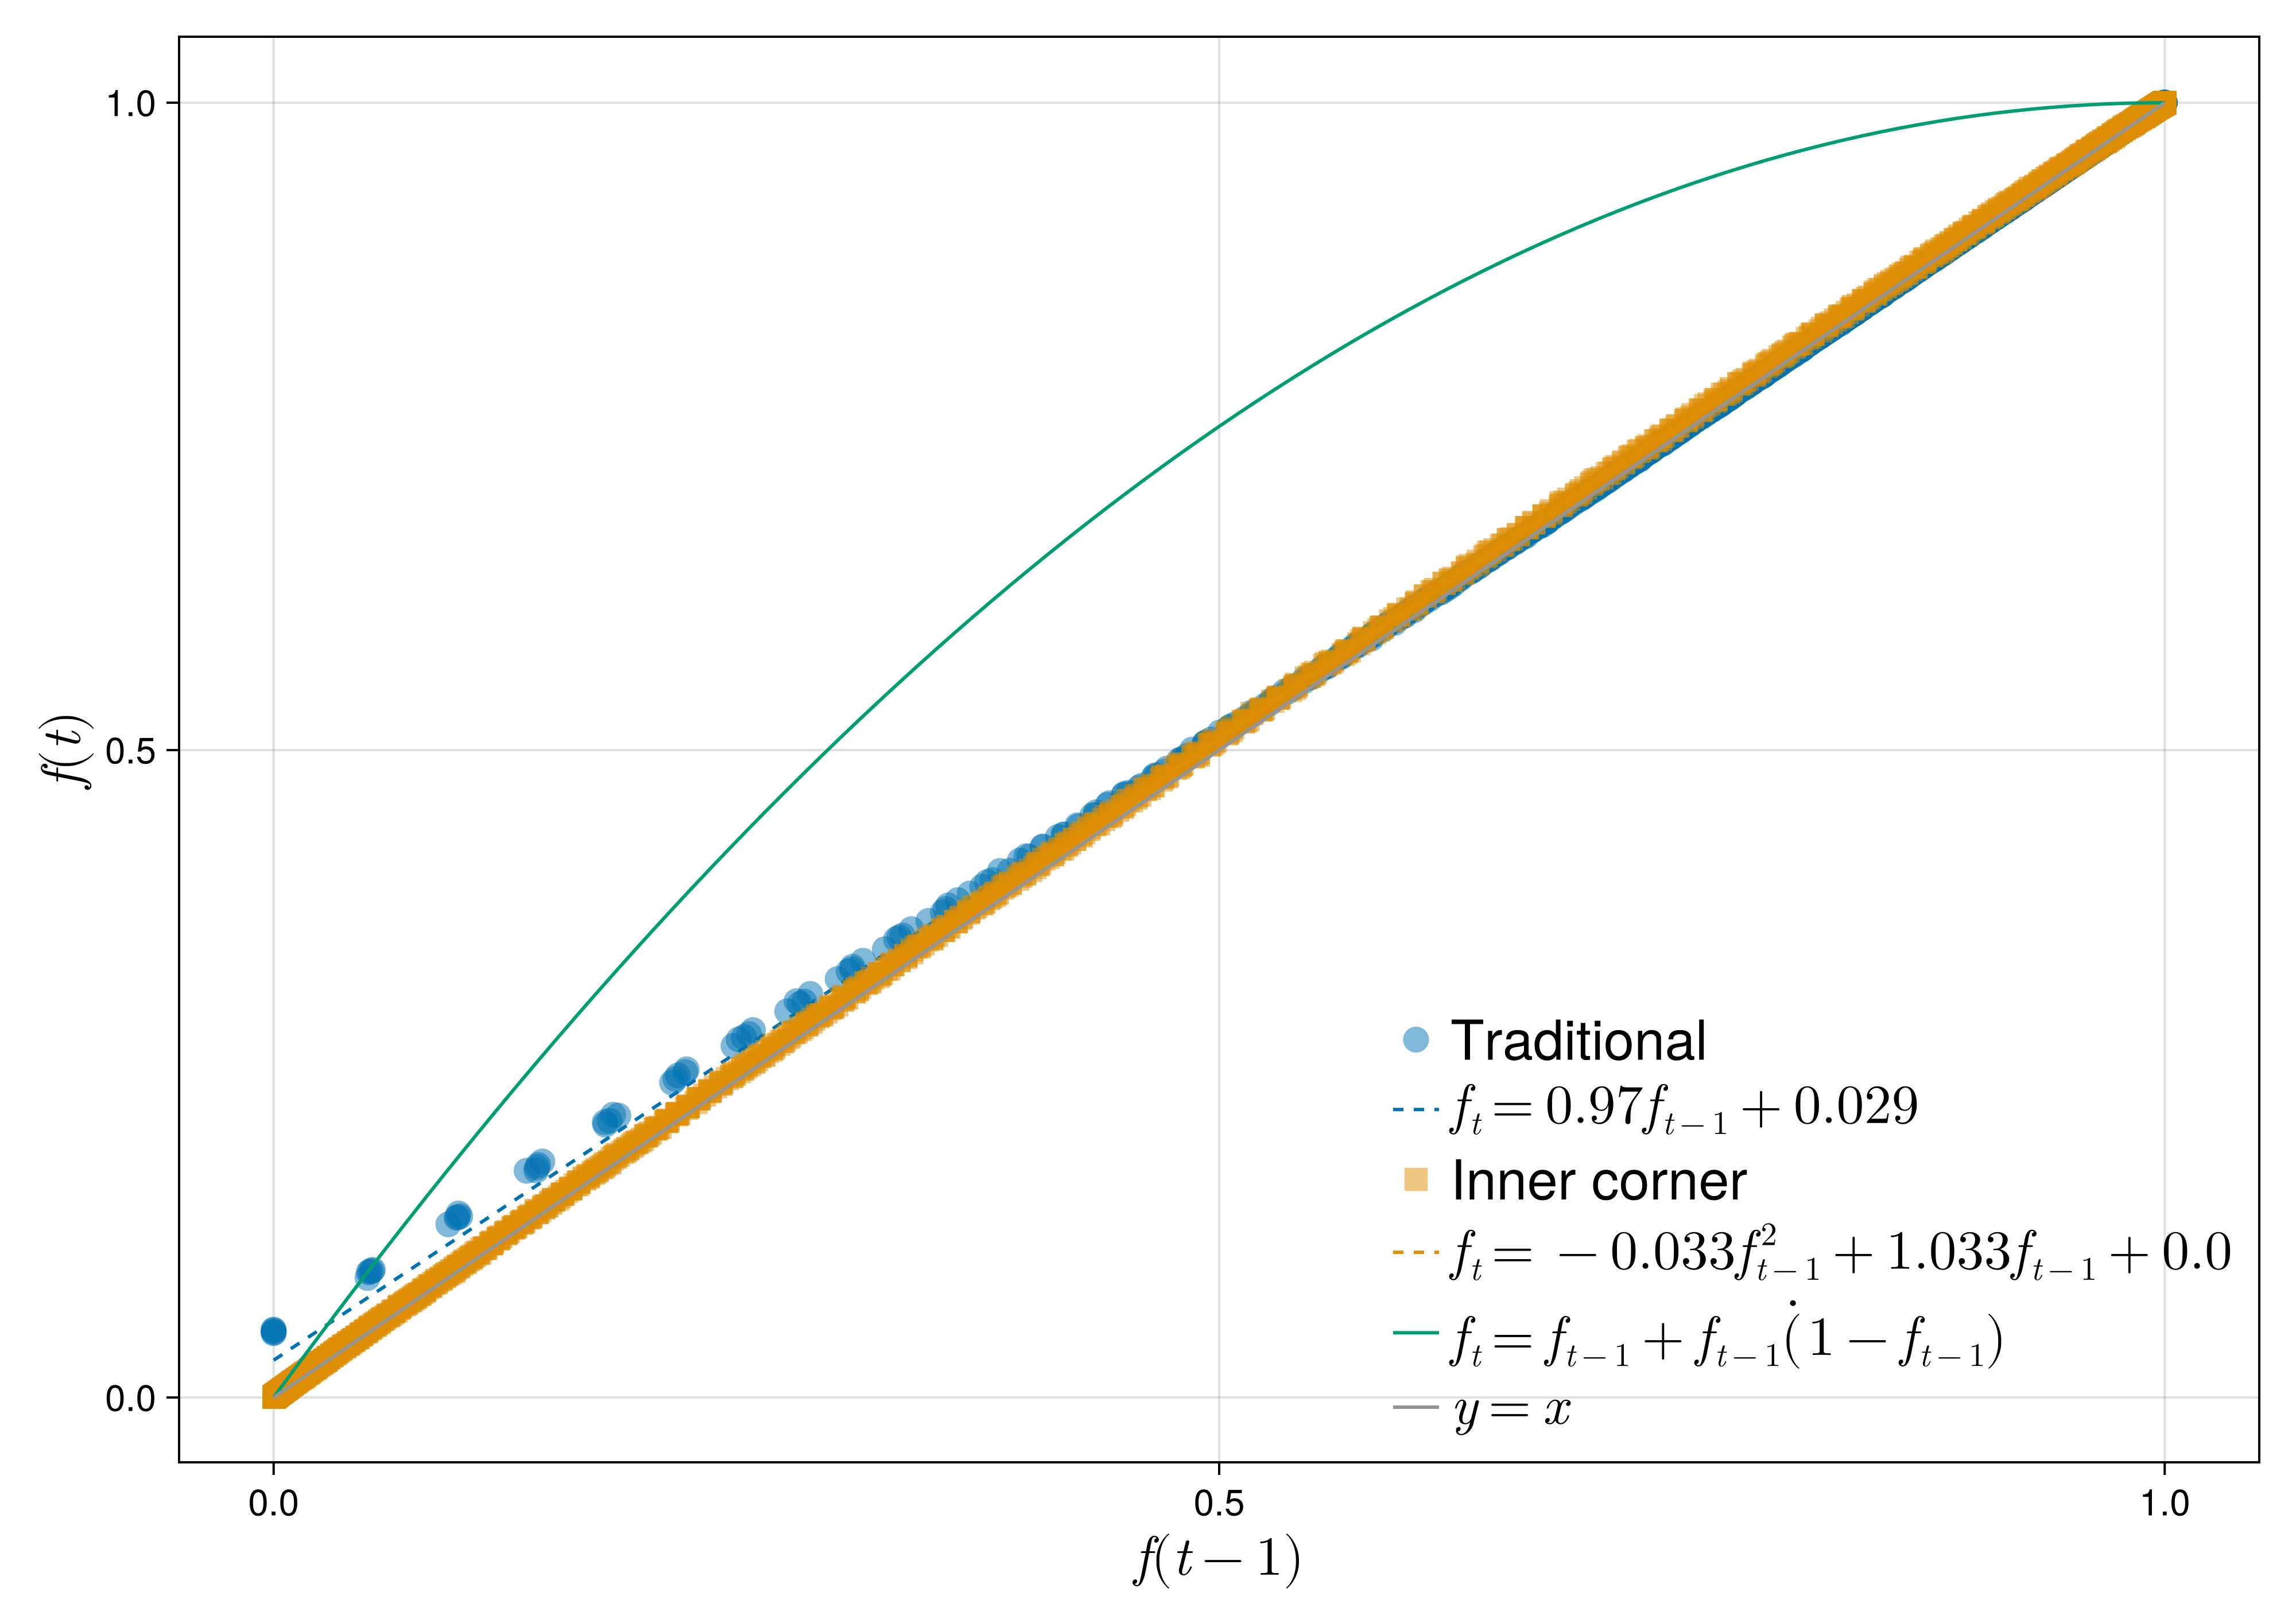
\includegraphics[width=0.47\textwidth]{figures/2D-BPCAIH-analysis/return plots/return-map-128-0.1-0.5-0.4.png}}
            \subfigure[$L=32,\space\rho_0=9,\space\lambda=0.5\pm0.0$]{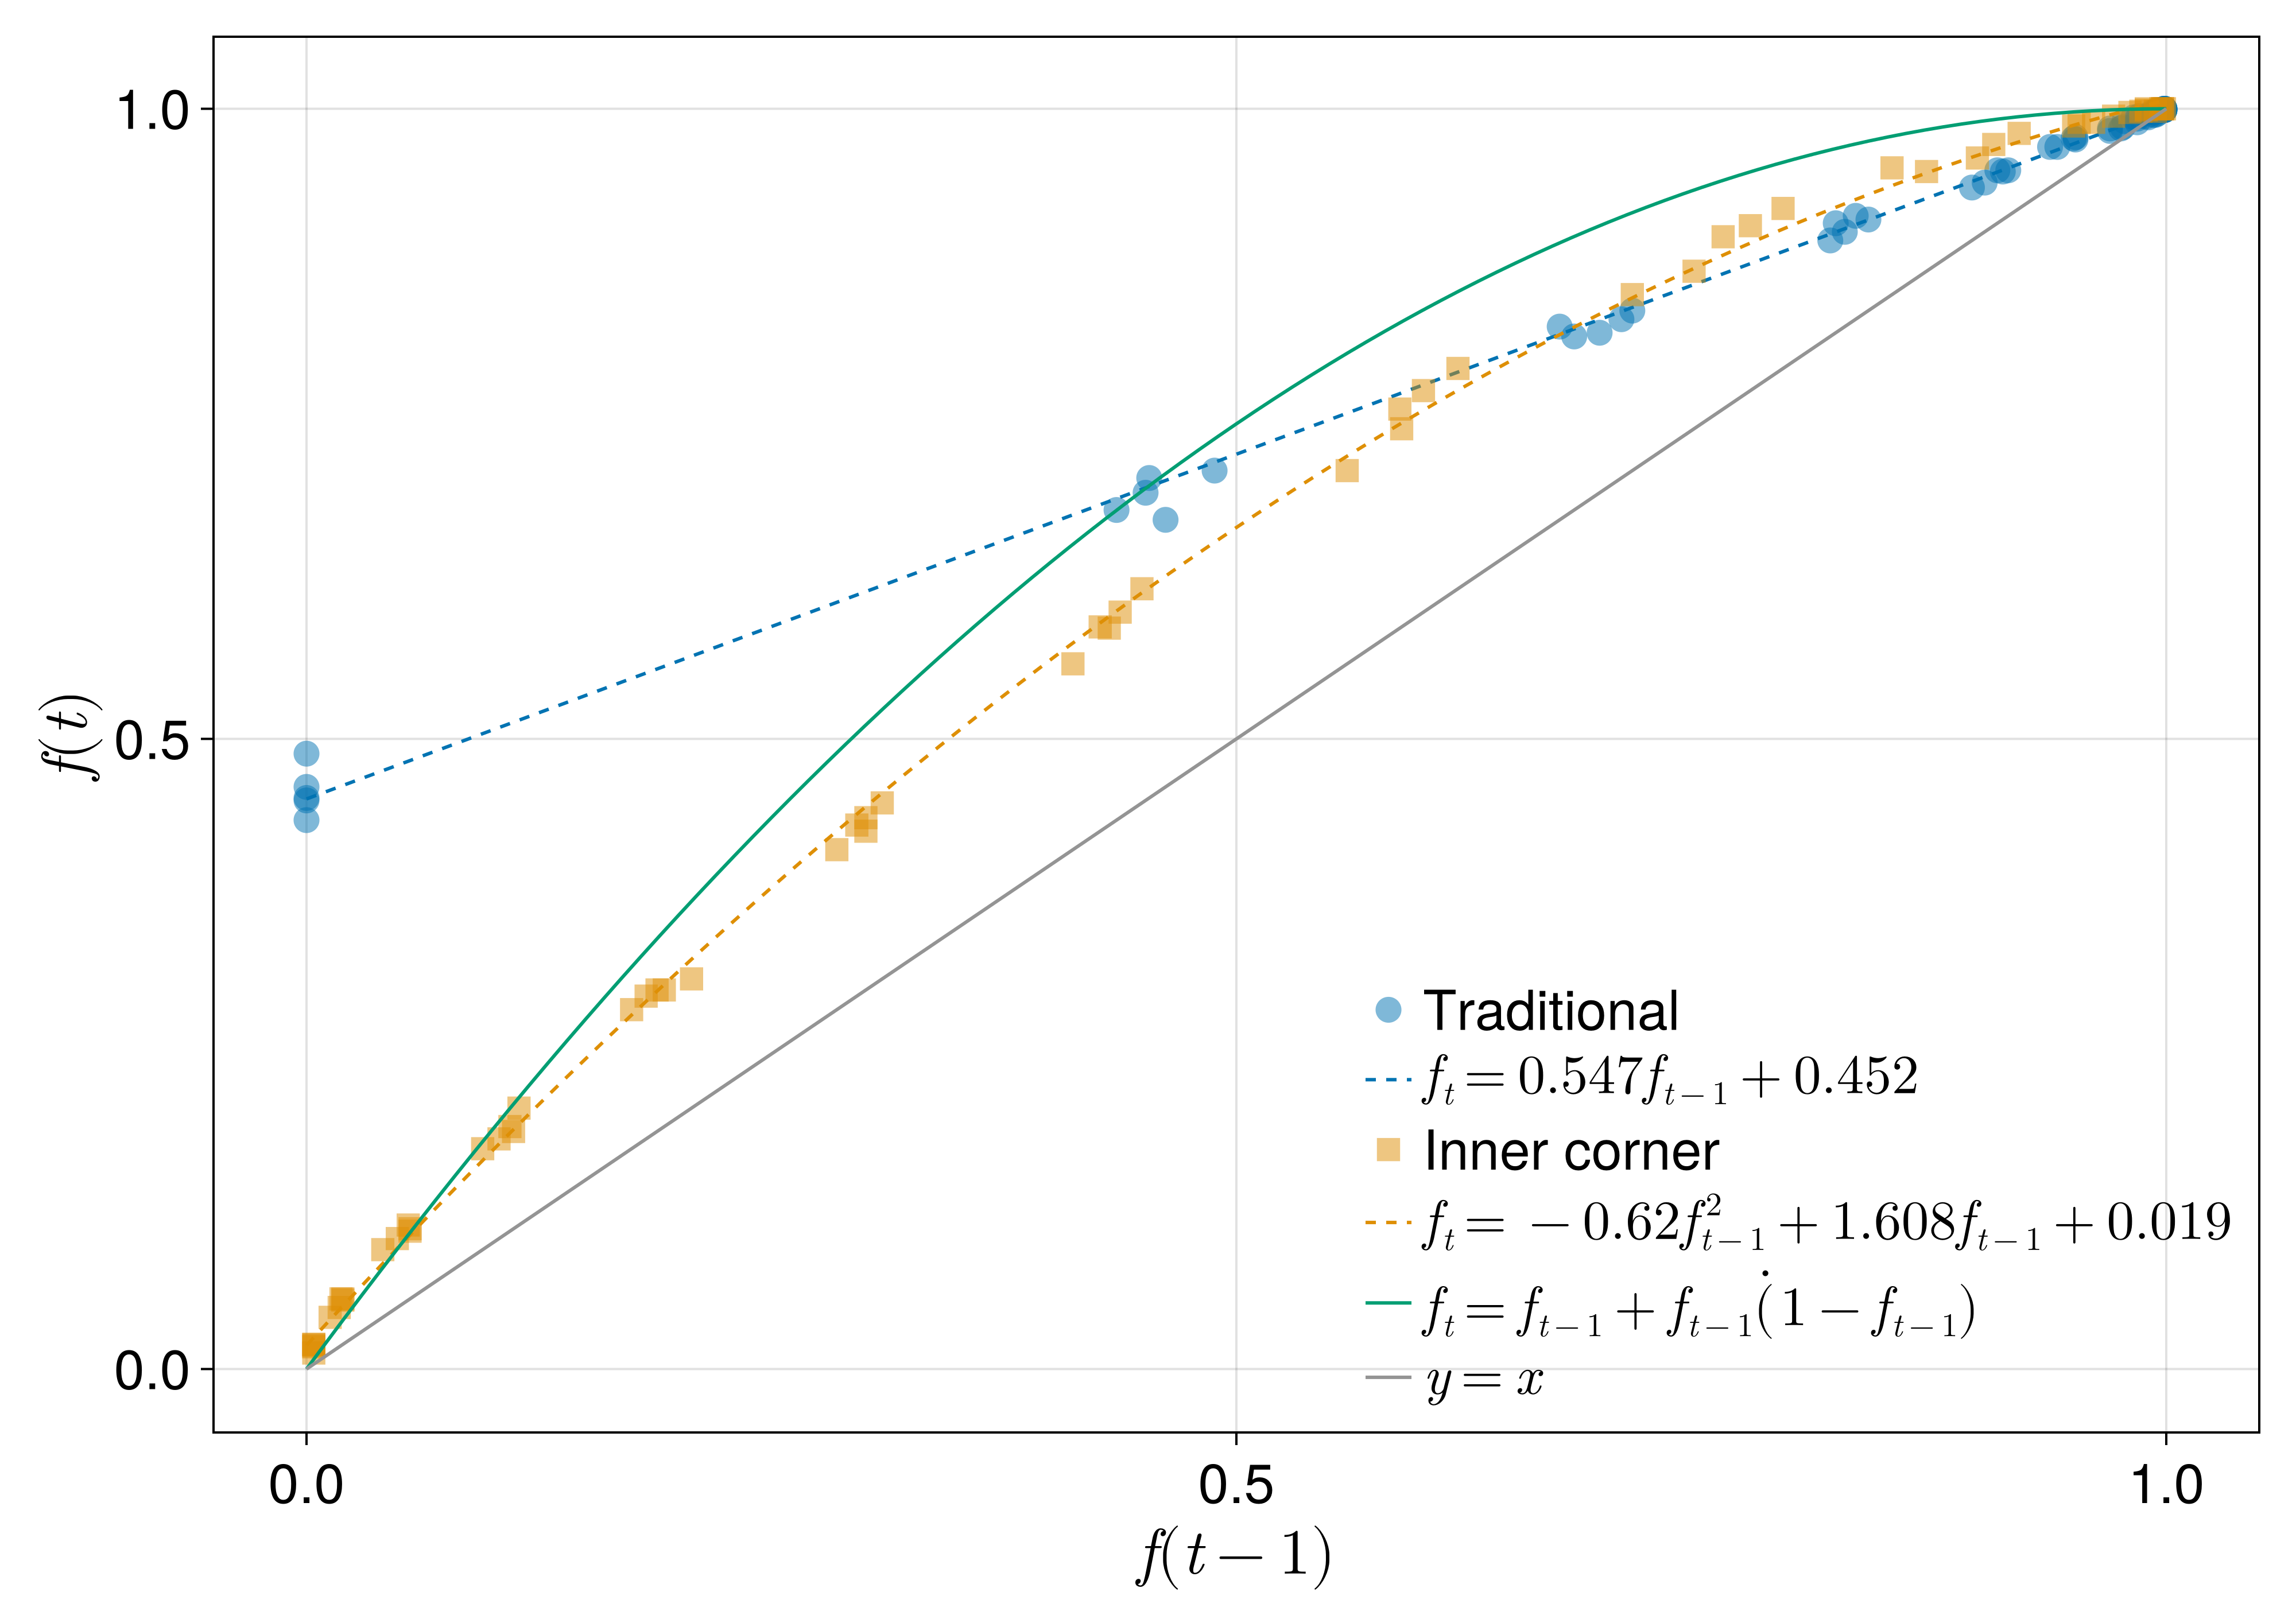
\includegraphics[width=0.47\textwidth]{figures/2D-BPCAIH-analysis/return plots/return-map-32-0.9-0.5-0.0.png}}
            \caption{Return map for selected parameter sets for both TI and PI.
            Blue circles represent the data points for TI and orange squares represent the data points for PI.
            The corresponding best-fit quadratic function obtained using the Levenberg-Marquardt algorithm for each set of data points are shown in blue and orange dashed lines respectively.
            The green line represents Nitta's theoretical model (Equation~\ref{eq: nitta model}) and the gray line represents $y=x$.}
            \label{fig:Return map}
        \end{figure}
        
        Comparing our data to Roxas' work \cite{roxas2010seating}, we find that the inner corner seating arrangement performs the best in our model, which is different from their findings where the outer corner seating arrangement performed the best.
        This difference can be attributed to the simplifications made in our model.
        We were not able to consider the aptitude similarity effect that happens where students of similar aptitude learn better when grouped together regardless of their actual aptitude level \cite{smith2009peer}.
        The implementation of this phenomenon is better suited for a continuous-state model rather than a binary-state model.
        Additionally, we did not consider the orientation of the students in the classroom, resulting in an isotropic system.
        In addition to the findings regarding seating arrangements, our model also agrees with their findings that homogenous classes find better improvements compared to heterogeneous classes.
    
\section{Summary and Conclusion}
    We propose a probabilistic cellular automata model as a new way of investigating learning dynamics in the classroom.
    Through this model, we can investigate how different factors can affect students' learning in the classroom for both traditional instruction (TI) and peer instruction (PI).

    We found that TI performs better in larger classes and when the students have low learning rate heterogeneity.
    On the other hand, PI performs better in smaller classes and when the students have high learning rate heterogeneity.
    To be more precise, class size, heterogeneity, and low positional learning factor affect both TI and PI negatively, but TI is not as affected by class size compared to PI and PI is not as affected by heterogeneity compared to TI.

    We also found that when a highly heterogeneous class is under TI, the class exhibits a two-stage learning process where majority of the fast students learn in the first few time steps and the rest of the time is spend waiting for slower students to learn. Our findings regarding class heterogeneity are in line with those of Roxas, et al. (2010) \cite{roxas2010seating}.
    However, our findings regarding seating arrangement differ from theirs where they found that the outer corner seating arrangement perform best while we found that the inner corner seating arrangement perform best.
    This difference is likely because of the simplifications made in our model --- namely learning isotropy and non-implementation of an aptitude similarity effect.
    These simplifications are from the limitations of having a binary-state model.

    Another limitation of having a binary-state model is that we there is not much insight to be gained from tracking individual students' learning.
    Hence, we chose to track the class's learning as a whole.
    Despite having a different way to assess the methods of instruction effectiveness, our findings are consistent with the existing works like that of Nitta, et al. \cite{nitta2019mathematical} which is backed by real-world data.

    While our model can be a good approximation of the real world, there are still improvements that can be made.
    The current model only considers the peer discussion part of a whole PI session.
    A mixed model that considers the whole session with a mix of TI and TI would be a better representation of the real world.
    Additionally, transitioning to a continuous-state model would allow us to incorporate more real-world phenomena like aptitude similarity and orientation effects.


\bibliography{biblio}

\end{document}

